% =============================================================================================
%  Rapport scientifique — Imagine & Make 2026, défi Avelis, Bloc 3 « Flux logistiques et données »
%  Compilation : pdfLaTeX + Biber (Overleaf : compilateur pdfLaTeX, la bibliographie est
%  traitée automatiquement). Figures : rapport/generer_figures.py (données du logiciel).
% =============================================================================================
\documentclass[11pt,a4paper]{article}

\usepackage[utf8]{inputenc}
\usepackage[T1]{fontenc}
\usepackage[french]{babel}
\usepackage{amsmath}
\usepackage{newtxtext,newtxmath}
\usepackage[a4paper,top=2.2cm,bottom=2.4cm,left=2.2cm,right=2.2cm]{geometry}
\usepackage{microtype}
\usepackage{graphicx}
\usepackage{booktabs}
\usepackage{tabularx}
\usepackage{array}
\usepackage{xcolor}
\usepackage[font=small,labelfont=bf,labelsep=period]{caption}
\usepackage{subcaption}
\usepackage{enumitem}
\usepackage{eurosym}
\usepackage{csquotes}
\usepackage[backend=biber,style=numeric-comp,sorting=none,maxbibnames=6,giveninits=true]{biblatex}
\addbibresource{references.bib}
\usepackage[hidelinks]{hyperref}

\graphicspath{{figures/}{figures/captures/}}
\setlist{itemsep=1pt,topsep=3pt}
\renewcommand{\arraystretch}{1.15}
\newcolumntype{Y}{>{\raggedright\arraybackslash}X}

\newcommand{\EUR}{\,\euro}
\newcommand{\mdeux}{m\textsuperscript{2}}
\newcommand{\COdeux}{CO\textsubscript{2}}
\newcommand{\hyp}{\textsuperscript{\textsf{H}}}
\newcommand{\code}[1]{\texttt{#1}}

\title{\vspace{-1.2cm}\textbf{Flux logistiques, implantation \emph{lean} et jumeau numérique
supervisé d'une usine de construction hors site à 1\,500~logements par an}\\[4pt]
\large Le cas de l'usine Avelis de Torcy (Saône-et-Loire)}
\author{Équipe Bloc~3 \enquote{Flux logistiques et données}\\
\small Imagine \& Make 2026 --- défi Avelis}
\date{Novembre 2026}

\begin{document}
\maketitle

\begin{abstract}
\noindent La construction hors site promet de lever la stagnation de productivité du bâtiment,
mais elle déplace le problème : la cadence visée par Avelis (1\,000 à 1\,500 logements par an
en 2029) ne sera tenue que si les flux physiques, le foncier et les données suivent les cellules
robotisées. Nous traitons ce problème comme un système unique, du camion fournisseur au convoi
de livraison. Un modèle analytique (takt, ressources, surfaces, réseau) et une simulation à
événements discrets reproductible dimensionnent la chaîne et comparent trois implantations sur le
foncier de Torcy. Une implantation optimisée selon les principes \emph{lean} réduit de 15\,\% la
distance d'un sous-ensemble, de 48\,\% celle de la gamme des murs et de 28\,\% la distance
parcourue en charge, sans croisement de flux, alors que le débit reste fixé par le goulot
d'assemblage 3D (12~baies chargées à 85\,\%). Nous proposons ensuite un jumeau numérique alimenté
par le scan des pièces, qui place l'humain dans la boucle de décision : il propose, l'opérateur
valide. Sa prévision des fins de fabrication réduit l'erreur absolue moyenne de 34\,\% par
rapport à une prévision naïve, et il isole un poste ralenti dès trois passages. Deux cas
d'application, l'hébergement modulaire des salariés des grands chantiers nucléaires de Gravelines
et de Flamanville, puis un programme urbain dans la métropole de Lyon, montrent que le bon schéma
industriel dépend de la géographie de la demande : usine unique pour une demande diffuse ou proche,
usine mère et unités d'assemblage foraines dès 900 à 1\,100 logements par an pour une demande
lointaine et concentrée, avec 70\,\% d'émissions de transport en moins.

\medskip\noindent\textbf{Mots-clés :} construction hors site ; \emph{lean manufacturing} ;
implantation d'usine ; simulation à événements discrets ; traçabilité ; jumeau numérique ;
Industrie~5.0 ; humain dans la boucle.
\end{abstract}

% =============================================================================================
\section{Introduction}
% =============================================================================================

La construction est l'un des secteurs dont la productivité a le moins progressé au cours des
dernières décennies : de l'ordre de 1\,\% par an à l'échelle mondiale, contre près de 3\,\% pour
l'ensemble de l'économie et davantage pour l'industrie manufacturière~\cite{barbosa2017}.
L'industrialisation hors site, qui transfère en usine la fabrication d'éléments 1D (ossatures),
2D (murs, planchers), 3D (modules volumiques) et de pods techniques, est l'une des réponses les plus
étudiées~\cite{gibb1999,lawson2014,bertram2019}. Elle offre une qualité plus régulière, des délais
de chantier plus courts et un meilleur bilan sur le cycle de vie, notamment par la réutilisation
des modules~\cite{kamali2016}. Elle n'est pourtant pas un simple déplacement du chantier vers
l'atelier : passer d'une logique de projet à une logique de produit suppose de maîtriser des
flux répétitifs, une cadence et des données~\cite{bertram2019}.

Avelis, groupe français de construction hors site, veut passer d'une fabrication artisanale à un
modèle industriel standardisé et automatisé, capable de 1\,000 à 1\,500 logements par an en 2029,
sur son site de Torcy (Saône-et-Loire) : 42\,786~\mdeux{} d'emprise actuelle et 27\,443~\mdeux{}
d'extension possible~\cite{imaginemake2026}. Le défi Imagine \& Make demande de concevoir la chaîne
industrielle robotisée correspondante, en définissant la juste place de l'humain. Il est
organisé en trois blocs : conception (Bloc~1), production robotisée (Bloc~2), flux logistiques
et données (Bloc~3). Ce rapport présente le travail du Bloc~3.

\paragraph{Contributions.} \emph{(i)}~Une vision d'ensemble chiffrée de la chaîne : schéma
industriel, cadence, implantation, feuille de route et place de l'humain (section~\ref{sec:vision}).
\emph{(ii)}~Un état de l'art croisant construction hors site, \emph{lean}, implantation, simulation,
traçabilité et jumeaux numériques (section~\ref{sec:etat}). \emph{(iii)}~Une méthode de
dimensionnement et une implantation optimisée sur le foncier réel de Torcy, évaluées par simulation
(sections~\ref{sec:methode} et~\ref{sec:resultats}). \emph{(iv)}~Un jumeau numérique supervisé,
réellement alimenté par le scan des pièces sur une maquette, avec deux briques d'apprentissage
statistique dont la précision est mesurée (section~\ref{sec:jumeau}). \emph{(v)}~Deux cas
d'application qui éprouvent le choix du schéma industriel (section~\ref{sec:cas}).

\paragraph{Convention.} Avelis ne mesurant pas encore ses flux (la fabrication est aujourd'hui
manuelle et non scannée), la plupart des paramètres sont des hypothèses. Chacune est marquée
\enquote{H} dans le modèle et modifiable dans le logiciel ; seules les données fournies par Avelis
sont marquées \enquote{A}. Aucune hypothèse n'a été ajustée pour atteindre un résultat attendu ;
les écarts sont expliqués. Les résultats valent donc par leur structure et leurs ordres de
grandeur plus que par leurs décimales.

% =============================================================================================
\section{Vision d'ensemble de la chaîne}\label{sec:vision}
% =============================================================================================

\paragraph{Cadence.} À 1\,500 logements par an et 1,2~module par logement\hyp{}, sur 220~jours
ouvrés et deux équipes de 8~heures (hypothèses communes aux trois blocs), l'usine doit sortir
8,18~modules et 6,82~pods par jour. Avec un taux de rendement synthétique (TRS) de 80\,\%\hyp{},
le temps net quotidien est de 768~min et le takt module vaut 93,9~min (équation~\eqref{eq:takt}).
Toute la chaîne se dimensionne à partir de cette pulsation.

\paragraph{Schéma industriel.} Deux schémas sont possibles : une usine unique qui expédie des
modules finis, ou une usine mère très automatisée qui fabrique les sous-ensembles (murs et pods)
et les envoie en kits à des usines satellites d'assemblage proches des régions. La
section~\ref{sec:cas} montre que la réponse dépend de la géographie de la demande. Pour une
demande nationale diffuse, l'usine unique est la moins chère jusqu'à 4\,700 logements par an
(tableau~\ref{tab:reseaux}). \textbf{Nous retenons donc l'usine unique sur le foncier de Torcy
agrandi de son extension}, complétée, pour des programmes lointains et concentrés, par des unités
d'assemblage foraines temporaires.

\paragraph{Feuille de route d'automatisation.} Nous proposons une montée en charge par paliers,
cohérente avec celle du Bloc~2, plutôt qu'une robotisation complète dès le départ. Les données de
flux sont rares aujourd'hui ; chaque palier doit donc produire les mesures qui justifient le
suivant :
\begin{itemize}
  \item \textbf{Palier 0 (2026--2027)} : marquage QR de chaque pièce, scan manuel au téléphone,
        jumeau en mode \enquote{ombre} et en mode proposition. C'est l'état de notre démonstrateur.
  \item \textbf{Palier 1 (2028)} : ligne 2D robotisée et lecteurs RFID fixes aux cinq nœuds
        de flux (réception, kitting, sorties de lignes, contrôle final, expédition) ; AGV pour les
        lots, kits et pods.
  \item \textbf{Palier 2 (2029)} : cadence de 1\,500 logements par an, 12~baies d'assemblage,
        jumeau recalé sur des données réelles et prévisions de fin de fabrication en
        production.
  \item \textbf{Palier 3 (au-delà de 2030)} : seconde ligne 2D et seconde ligne pods dans la
        réserve foncière prévue à cet effet ; unités foraines pour les grands programmes.
\end{itemize}

\paragraph{Place de l'humain.} Nous suivons la typologie des niveaux d'automatisation de
Parasuraman, Sheridan et Wickens~\cite{parasuraman2000} et la vision de l'Industrie~5.0, centrée
sur l'humain~\cite{breque2021,xu2021}. Le tableau~\ref{tab:humain} résume la répartition des rôles.

\begin{table}[!htbp]
\centering\small
\caption{Place de l'humain dans la chaîne logistique et de données.}\label{tab:humain}
\begin{tabularx}{\linewidth}{@{}lYYY@{}}
\toprule
 & \textbf{L'humain intervient} & \textbf{L'humain est assisté} & \textbf{L'humain n'intervient plus} \\
\midrule
Flux physiques & réception qualitative des lots, retouches, assemblage 3D (finitions) &
préparation des kits (consignes au téléphone), conduite des porteurs &
transfert des lots, kits et pods (AGV) \\
Données & déclaration d'un défaut et de sa cause, choix du chantier à l'expédition &
contrôle de séquence (étape refusée hors gamme), alertes kanban &
horodatage, calcul des durées, mise à jour du plan \\
Décision & validation, modification ou rejet de chaque consigne proposée &
prévision des fins de fabrication, détection des postes lents &
aucune décision n'est appliquée sans validation \\
\bottomrule
\end{tabularx}
\end{table}

\paragraph{Organisation : du projet au processus.} Le passage d'une logique de projet (un
bâtiment, une équipe) à une logique de processus (un flux, un takt) est au c\oe ur du
\emph{lean}~\cite{womack1996,liker2004}. Il se traduit par :
\begin{itemize}
  \item un responsable de chaîne de valeur, de la réception à l'expédition ;
  \item une revue de performance quotidienne au pied des lignes, appuyée sur les tuiles du jumeau
        (terminés face à l'objectif, en-cours, défauts, lots bloqués) ;
  \item des indicateurs mesurés automatiquement plutôt que déclarés : débit, délai de l'ordre de
        fabrication (OF) au stock de produits finis, part tracée de bout en bout, délai
        d'affichage d'un événement.
\end{itemize}

\paragraph{Interfaces avec les autres blocs.} Le tableau~\ref{tab:interfaces} explicite ce que le
Bloc~3 reçoit des Blocs~1 et~2 et ce qu'il leur fournit. La gouvernance stratégique et la
cybersécurité sont hors périmètre ; nous signalons seulement que l'API de scan, aujourd'hui sans
authentification sur un réseau local, devra être durcie selon la série IEC~62443~\cite{iec62443}
avant tout déploiement.

\begin{table}[!htbp]
\centering\small
\caption{Interfaces du Bloc~3 avec les Blocs~1 (conception) et~2 (production).}\label{tab:interfaces}
\begin{tabularx}{\linewidth}{@{}lYY@{}}
\toprule
 & \textbf{Le Bloc~3 reçoit} & \textbf{Le Bloc~3 fournit} \\
\midrule
Bloc~1 & nomenclature par module (BOM), identifiants des pièces, gabarits (module 3,5\,$\times$\,10\,m),
  ordres de fabrication & contenu des kits, contraintes de transport (catégorie de convoi),
  retours qualité par cause \\
Bloc~2 & temps de cycle par poste, taux de panne (MTBF/MTTR), états des machines &
  takt, séquence de lancement, kits à l'heure, consignes validées, durées réelles mesurées \\
\bottomrule
\end{tabularx}
\end{table}

% =============================================================================================
\section{Verrous scientifiques}\label{sec:verrous}
% =============================================================================================

\begin{description}[leftmargin=0pt,itemsep=3pt]
\item[V1 --- Dimensionner sous incertitude.] Les temps de cycle, les retards fournisseurs, les
pannes et les défauts sont aléatoires. Un dimensionnement par les moyennes sous-estime les
files d'attente, car celles-ci croissent fortement quand la charge s'approche de 1~\cite{hopp2008}.
Il faut donc un modèle stochastique, reproductible, qui relie cadence, ressources et stocks.
\item[V2 --- Implanter sur un foncier contraint.] Le problème d'implantation est NP-difficile ;
sa forme quadratique remonte à Koopmans et Beckmann~\cite{koopmans1957,drira2007}. Ici, il
se double d'un foncier irrégulier, d'un accès unique et d'une extension qui n'est pas encore acquise.
\item[V3 --- Choisir le schéma de réseau.] Usine unique ou usine mère et satellites : c'est un
arbitrage entre coûts fixes et coûts de transport~\cite{melo2009}, compliqué par le transport
exceptionnel des modules volumiques~\cite{arrete2006}.
\item[V4 --- Tracer chaque composant.] La traçabilité de bout en bout exige que \emph{tous} les
points d'une gamme soient lus : la probabilité de trace complète décroît géométriquement avec le
nombre de points (équation~\eqref{eq:trace}). Une technologie de lecture médiocre rend la
traçabilité illusoire.
\item[V5 --- Synchroniser et décider avec peu de données.] Un jumeau numérique suppose un flux de
données fiable et des modèles qui apprennent. Or l'usine ne produit au départ que quelques
centaines d'événements. Les méthodes gourmandes en données sont alors inapplicables, et une
décision automatique non supervisée serait contraire à l'Industrie~5.0 et exposée aux
\enquote{ironies de l'automatisation}~\cite{bainbridge1983}.
\end{description}

% =============================================================================================
\section{État de l'art}\label{sec:etat}
% =============================================================================================

\paragraph{Construction hors site.} Gibb~\cite{gibb1999} distingue préfabrication, pré-assemblage et
modularisation ; Lawson et al.~\cite{lawson2014} formalisent la conception modulaire, du gabarit
transportable à l'assemblage. Kamali et Hewage~\cite{kamali2016} montrent, sur le cycle de vie,
des gains environnementaux liés à la réduction des déchets et à la réutilisation. Bertram et
al.~\cite{bertram2019} soulignent que la rentabilité dépend d'un volume répété et d'une logistique
de livraison maîtrisée, le transport de volumes encombrants pesant sur le coût final. C'est
l'arbitrage V3.

\paragraph{\emph{Lean manufacturing} et \emph{lean construction}.} Le système de production Toyota
repose sur deux piliers, le juste-à-temps et le \emph{jidoka}, ou autonomation : la machine s'arrête
et signale, l'humain résout~\cite{ohno1988}. Womack, Jones et Roos l'ont diffusé sous le nom de
\emph{lean}~\cite{womack1990}, puis en ont tiré cinq principes : valeur, chaîne de valeur, flux,
tirage, perfection~\cite{womack1996}. Le kanban matérialise le tirage~\cite{sugimori1977} ; la
cartographie de la chaîne de valeur (VSM) rend visibles les attentes et les
stocks~\cite{rother1999}. La loi de Little ($L = \lambda W$) relie l'en-cours, le débit et le
délai~\cite{little1961,hopp2008}. Pour la construction, Koskela~\cite{koskela1992} propose de voir
la production comme transformation, flux et valeur, et Ballard~\cite{ballard2000} en tire le
\emph{Last Planner System}. Avec l'usine hors site, la construction redevient un problème de flux
manufacturier, où le \emph{lean} s'applique presque littéralement.

\paragraph{Implantation d'usine.} La planification systématique de l'implantation (SLP) de
Muther~\cite{muther1961}, reprise dans les manuels de référence~\cite{tompkins2010}, enchaîne
analyse des flux, relations entre activités, besoins en surface et alternatives. Les formulations
d'optimisation (affectation quadratique, implantation en blocs, approches continues) sont
recensées par Drira et al.~\cite{drira2007}. Leurs critères dominants sont la distance pondérée
par les flux et l'absence de croisements, deux indicateurs que nous mesurons.

\paragraph{Simulation à événements discrets (SED).} La SED est l'outil de référence pour évaluer
des systèmes de production stochastiques~\cite{banks2010,law2015}. En construction, AbouRizk en
montre l'apport pour la planification et l'analyse des opérations~\cite{abourizk2010}. La SED
est aussi le \enquote{modèle} d'un jumeau numérique : elle donne la référence attendue à
laquelle comparer le réel.

\paragraph{Réseaux de production et de distribution.} La localisation d'installations dans une
chaîne logistique arbitre entre coûts fixes, coûts de transport et niveau de
service~\cite{melo2009}. Pour des modules de 3,5~m de large, la réglementation française classe le
convoi en deuxième catégorie de transport exceptionnel (largeur comprise entre 3 et
4~m)~\cite{arrete2006}. Cela impose autorisation, itinéraires et horaires contraints, alors
qu'un kit de murs voyage en semi-remorque standard.

\paragraph{Traçabilité.} La RFID permet une lecture sans contact, sans ligne de vue et en
masse~\cite{want2006}. Son intérêt en construction pour suivre les matériaux a été démontré par
Jaselskis et El-Misalami~\cite{jaselskis2003}. Le QR code (ISO/IEC~18004~\cite{iso18004}) est
quasi gratuit, mais demande un geste de scan par point. Le papier introduit délais et ressaisies.

\paragraph{Jumeaux numériques.} Grieves et Vickers définissent le jumeau comme la contrepartie
virtuelle d'un système physique, reliée à lui par des flux de données~\cite{grieves2017}.
Kritzinger et al.~\cite{kritzinger2018} distinguent, selon l'automatisation des échanges, trois
niveaux :
\begin{itemize}
  \item le \emph{modèle numérique}, avec des échanges manuels dans les deux sens ;
  \item l'\emph{ombre numérique}, avec un flux automatique du physique vers le virtuel seulement ;
  \item le \emph{jumeau}, avec des flux automatiques dans les deux sens.
\end{itemize}
Ils constatent que la plupart des travaux publiés sous le nom de jumeau sont en réalité des
modèles ou des ombres. Tao et al.~\cite{tao2019} et Negri et al.~\cite{negri2017} dressent l'état
de l'art industriel. En construction, Boje et al.~\cite{boje2020} et Sacks et al.~\cite{sacks2020}
appellent à des jumeaux qui bouclent sur la production (\enquote{plan, do, check, act}) plutôt
qu'à de simples maquettes numériques enrichies.

\paragraph{Industrie~5.0 et humain dans la boucle.} L'Industrie~5.0 replace l'humain, la
durabilité et la résilience au c\oe ur de l'industrie
numérique~\cite{breque2021,nahavandi2019,xu2021}. L'échelle de Parasuraman et al.~\cite{parasuraman2000}
situe le niveau où la machine \enquote{propose et exécute si l'humain approuve}. Bainbridge
rappelle qu'une automatisation trop complète dégrade la compétence et la vigilance de l'opérateur
au moment précis où l'on a besoin de lui~\cite{bainbridge1983}.

\paragraph{Statistique pour données rares.} La théorie de la crédibilité de Bühlmann~\cite{buhlmann1967}
pondère une moyenne observée et une valeur a priori selon le nombre d'observations. C'est un
estimateur de rétrécissement adapté au démarrage, quand les mesures sont rares. Pour détecter les
dérives, la médiane et l'écart absolu médian (MAD) résistent aux valeurs
aberrantes~\cite{rousseeuw1993,leys2013}, dans l'esprit de la maîtrise statistique des
procédés~\cite{montgomery2009}. Enfin, toute prévision doit être comparée à une référence
naïve~\cite{hyndman2021}.

\paragraph{Positionnement.} Aucun des travaux cités ne réunit, pour une usine hors site, le
dimensionnement analytique, la SED, l'implantation sur foncier réel, la traçabilité par
composant et un jumeau supervisé validé sur des données de scan. Notre contribution est cette
intégration, outillée et reproductible, plus qu'une avancée sur une brique isolée.

% =============================================================================================
\section{Méthode}\label{sec:methode}
% =============================================================================================

Le démonstrateur comprend deux logiciels. \code{avelis\_flux} est une application de bureau en
Python (modèle analytique, SED, interface, jumeau). \code{avelis\_scan} est un serveur de scan
avec une base SQLite, utilisé depuis un téléphone. Seules la bibliothèque standard,
\code{matplotlib}, \code{numpy} et \code{pillow} sont utilisées ; tout l'aléa passe par un
générateur à graine, ce qui rend chaque résultat reproductible. Nous ne décrivons ici que les
modèles ; les choix logiciels sont secondaires.

\subsection{Modèle analytique de dimensionnement}

Pour une cadence $L$ (logements/an), $n_m$ modules par logement et $J$ jours ouvrés, le débit
journalier et le takt module sont
\begin{equation}\label{eq:takt}
q_m = \frac{L\,n_m}{J}, \qquad T_t = \frac{H_o \cdot \mathrm{TRS}}{q_m},
\end{equation}
où $H_o = 960$~min est le temps d'ouverture quotidien. Le nombre de ressources d'un poste de
cycle $c_r$ est
\begin{equation}\label{eq:ressources}
N_r = \left\lceil \frac{c_r}{T_t\,\rho_{\max}} \right\rceil, \qquad
\rho_r = \frac{c_r}{T_t\,N_r},
\end{equation}
avec $\rho_{\max} = 0{,}90$\hyp{} la charge maximale admise. Les surfaces découlent des
ressources (surface unitaire $\times$ coefficient de circulation de 1,5\hyp) et des
couvertures de stock (matières : 10~jours ; produits finis : 5~jours). Les quais découlent du
nombre de camions et de leur temps d'occupation, avec un quai de secours.

\subsection{Modèle de réseau}

Pour chaque chantier $j$ de part de demande $p_j$, l'option A livre en convoi direct depuis
Torcy, l'option B livre en semi-remorque (3~kits) jusqu'au satellite le plus proche, puis en
convoi. Le coût logistique annuel est
\begin{equation}\label{eq:reseau}
C = M \sum_j p_j \sum_{t \in \mathcal{I}_j} \frac{d_t\,\kappa_t\,c_t}{u_t} + S\,F,
\end{equation}
où $M$ est le nombre de modules par an, $\mathcal{I}_j$ l'itinéraire du chantier $j$, $d_t$ la
distance routière (distance orthodromique $\times\,1{,}3$\hyp), $\kappa_t$ le coefficient de
retour (2 à vide pour un convoi, 1,6 pour un semi), $c_t$ le coût kilométrique (3,4 ou
1,9\EUR/km\hyp), $u_t$ les unités par véhicule, $S$ le nombre de satellites et $F$ leur coût
fixe annuel (9~M\EUR{} amortis sur 15~ans, plus 1,4~M\EUR/an\hyp). Les émissions de \COdeux{}
sont proportionnelles aux kilomètres facturés (1~kg/km\hyp). Le point de bascule est la plus petite
cadence pour laquelle $C_B < C_A$.

\subsection{Simulation à événements discrets}

La SED représente, minute par minute de temps d'ouverture, les objets suivants :
\begin{itemize}
  \item les camions fournisseurs : arrivées régulières, 12\,\% de retards, attente de quai,
        déchargement selon une loi triangulaire ;
  \item les lots : 6\,\% non conformes ;
  \item les ordres de fabrication : un toutes les 117~min ;
  \item le kitting : rupture signalée si le stock est vide ;
  \item la ligne 2D : pannes exponentielles de MTBF 2\,400~min ;
  \item les quatre postes en série de la ligne pods, avec défauts propres à chaque poste et
        surcroît de défauts au poste \enquote{parois} quand le lot est non conforme ;
  \item l'assemblage 3D (12~baies), le contrôle final (2\,\% de défauts), le stock de produits
        finis et les convois d'expédition.
\end{itemize}

Les transports internes (AGV, porteurs) suivent les chemins en L du plan. Le kit 2D part du
kitting avec un retard calculé pour arriver à l'assemblage en même temps que le pod : c'est une
synchronisation au sens du juste-à-temps. Chaque événement est enregistré par la technologie de
traçabilité simulée, avec un taux de lecture et un délai d'affichage qui lui sont propres. Pour
chaque pièce, la probabilité de trace complète est
\begin{equation}\label{eq:trace}
P_{\text{trace}} = \pi\,\tau^{\,k_m+k_p} + (1-\pi)\,\tau^{\,k_m},
\end{equation}
où $\tau$ est le taux de lecture, $k_m$ et $k_p$ les nombres de points obligatoires des gammes
module et pod, et $\pi = 0{,}83$ la proportion de modules avec pod. La simulation est vérifiée
de trois façons :
\begin{itemize}
  \item par 20~tests intégrés : moteur, conservation des pièces, reproductibilité,
        indépendance du flux physique vis-à-vis de la technologie ;
  \item par la confrontation de la part tracée simulée à l'équation~\eqref{eq:trace}, sur
        20~graines ;
  \item par la loi de Little (section~\ref{sec:resultats}).
\end{itemize}

\subsection{Implantations comparées}

Les trois implantations utilisent le contour réel du foncier, reconstitué à partir du plan
d'emprise (aires à 0,3\,\% des valeurs Avelis par la formule du lacet), l'accès poids lourds unique
à l'est et une voirie interne.
\begin{itemize}
  \item L'implantation \emph{actuelle} se limite au site existant ; ses quais sont partagés
        entre réception et expédition.
  \item L'implantation \emph{proposée} utilise l'extension avec un flux en U.
  \item L'implantation \emph{optimisée} suit une démarche SLP~\cite{muther1961} :
  \begin{itemize}
    \item zones ramenées à la taille du besoin ;
    \item lignes 2D et pods accolées à l'ouest de la halle d'assemblage, qui est le goulot ;
    \item lignes superposées, de sorte que leurs chemins ne se croisent pas ;
    \item bureaux déplacés à l'accueil ;
    \item expédition placée au droit du stock de produits finis ;
    \item réserve foncière dédiée aux lignes de 2030.
  \end{itemize}
\end{itemize}

% =============================================================================================
\section{Résultats : dimensionnement et implantation \emph{lean}}\label{sec:resultats}
% =============================================================================================

\subsection{Le goulot est l'assemblage 3D}

\begin{figure}[!htbp]
\centering
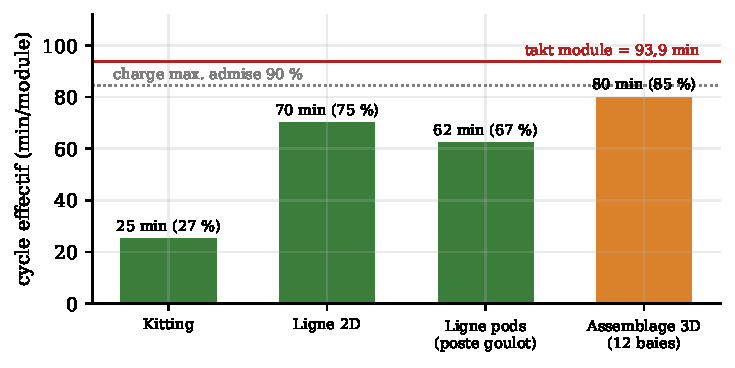
\includegraphics[width=0.78\linewidth]{yamazumi.pdf}
\caption{Diagramme Yamazumi à 1\,500 logements/an : cycle effectif par module (cycle divisé par le
nombre de ressources) face au takt de 93,9~min. L'assemblage 3D (960~min de travail, 12~baies)
est le goulot, chargé à 85\,\%.}\label{fig:yamazumi}
\end{figure}

\begin{table}[!htbp]
\centering\small
\caption{Dimensionnement à 1\,500 logements/an (usine unique). Valeurs du modèle analytique.}\label{tab:dim}
\begin{tabular}{@{}lr@{\hspace{2.5em}}lr@{}}
\toprule
Modules / pods par jour & 8,18 / 6,82 & Camions entrants par jour & 5,84 \\
Takt module / pod (min) & 93,9 / 112,6 & Convois sortants par jour & 8,18 \\
Baies d'assemblage 3D & 12 (85\,\%) & Quais réception / expédition & 2 / 2 \\
Lignes 2D / lignes pods & 1 (75\,\%) / 1 (67\,\%) & Surface nécessaire & 22\,864~\mdeux \\
Postes de kitting & 1 (27\,\%) & Utilisable : site seul / avec extension & 25\,672 / 42\,137~\mdeux \\
\bottomrule
\end{tabular}
\end{table}

Le tableau~\ref{tab:dim} et la figure~\ref{fig:yamazumi} montrent que la ligne 2D (70~min),
la ligne pods (75~min au poste goulot) et le kitting tiennent le takt avec une seule unité.
L'assemblage 3D, avec 16~heures de travail par module, impose 12~baies : il fixe la surface de la
halle et plafonne la cadence. La surface nécessaire en usine unique (22\,864~\mdeux) tient sur le
site seul (25\,672~\mdeux{} utilisables) à 1\,500 logements par an, mais la cadence maximale
admissible sans extension est de 1\,800 logements par an, contre plus de 3\,000 avec l'extension.
\textbf{L'extension est donc la condition de l'évolutivité}, plus que de la cadence 2029.

\subsection{Comparaison des implantations}

\begin{table}[!htbp]
\centering\small
\caption{Trois implantations, usine unique, 1\,500 logements/an, 10~jours simulés, graine 42.
Distances de manutention calculées sur le plan ; autres indicateurs issus de la SED.}\label{tab:implantations}
\begin{tabular}{@{}lrrr@{}}
\toprule
 & Actuelle (site seul) & Proposée (flux en U) & \textbf{Optimisée} \\
\midrule
Distance d'un sous-ensemble, pod + module (m) & 1\,018 & 681 & \textbf{580} \\
Gamme 2D, kitting $\rightarrow$ assemblage (m) & 177 & 343 & \textbf{177} \\
Croisements de flux & 2 & 0 & \textbf{0} \\
Distance parcourue en charge (km / 10~j) & 84,9 & 74,8 & \textbf{54,0} \\
Ruptures, attentes et blocages & 10 & 6 & \textbf{4} \\
Délai OF $\rightarrow$ stock PF moyen (h) & 23,6 & 23,5 & \textbf{22,9} \\
En-cours moyen (modules) & 11,2 & 11,2 & \textbf{11,0} \\
Taux d'atteinte de l'objectif & 99,3\,\% & 99,3\,\% & 99,3\,\% \\
\bottomrule
\end{tabular}
\end{table}

\begin{figure}[!htbp]
\centering
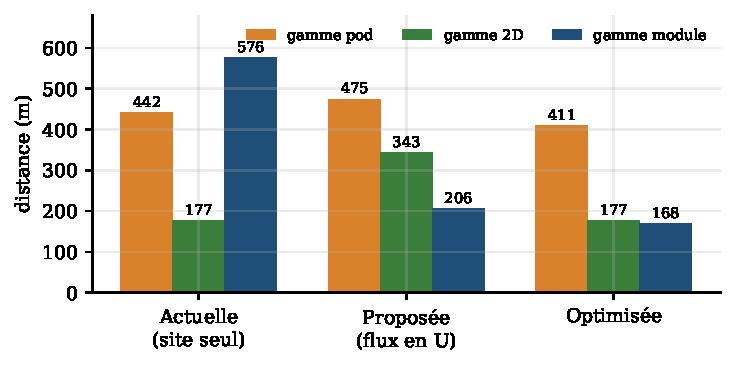
\includegraphics[width=0.72\linewidth]{distances_implantations.pdf}
\caption{Distance de manutention par gamme et par implantation (m).}\label{fig:distances}
\end{figure}

L'implantation optimisée réduit la distance d'un sous-ensemble de 15\,\% par rapport à la
proposée et de 43\,\% par rapport à l'actuelle ; elle divise par deux la gamme des murs
(tableau~\ref{tab:implantations}, figure~\ref{fig:distances}). Sur dix jours, elle économise
28\,\% des distances parcourues en charge, donc autant de temps d'AGV et de porteurs, d'énergie et
de risques de collision. En revanche, \textbf{le débit est identique dans les trois cas}
(8,12~modules/jour, soit 99,3\,\% de l'objectif). C'est le résultat attendu de la théorie des
contraintes : l'implantation agit sur le gaspillage de transport, pas sur le goulot.
Améliorer la cadence suppose d'agir sur l'assemblage 3D lui-même, en réduisant le travail par
module ou en ajoutant des baies, ce qui relève de l'interface avec le Bloc~2.

\begin{figure}[!htbp]
\centering
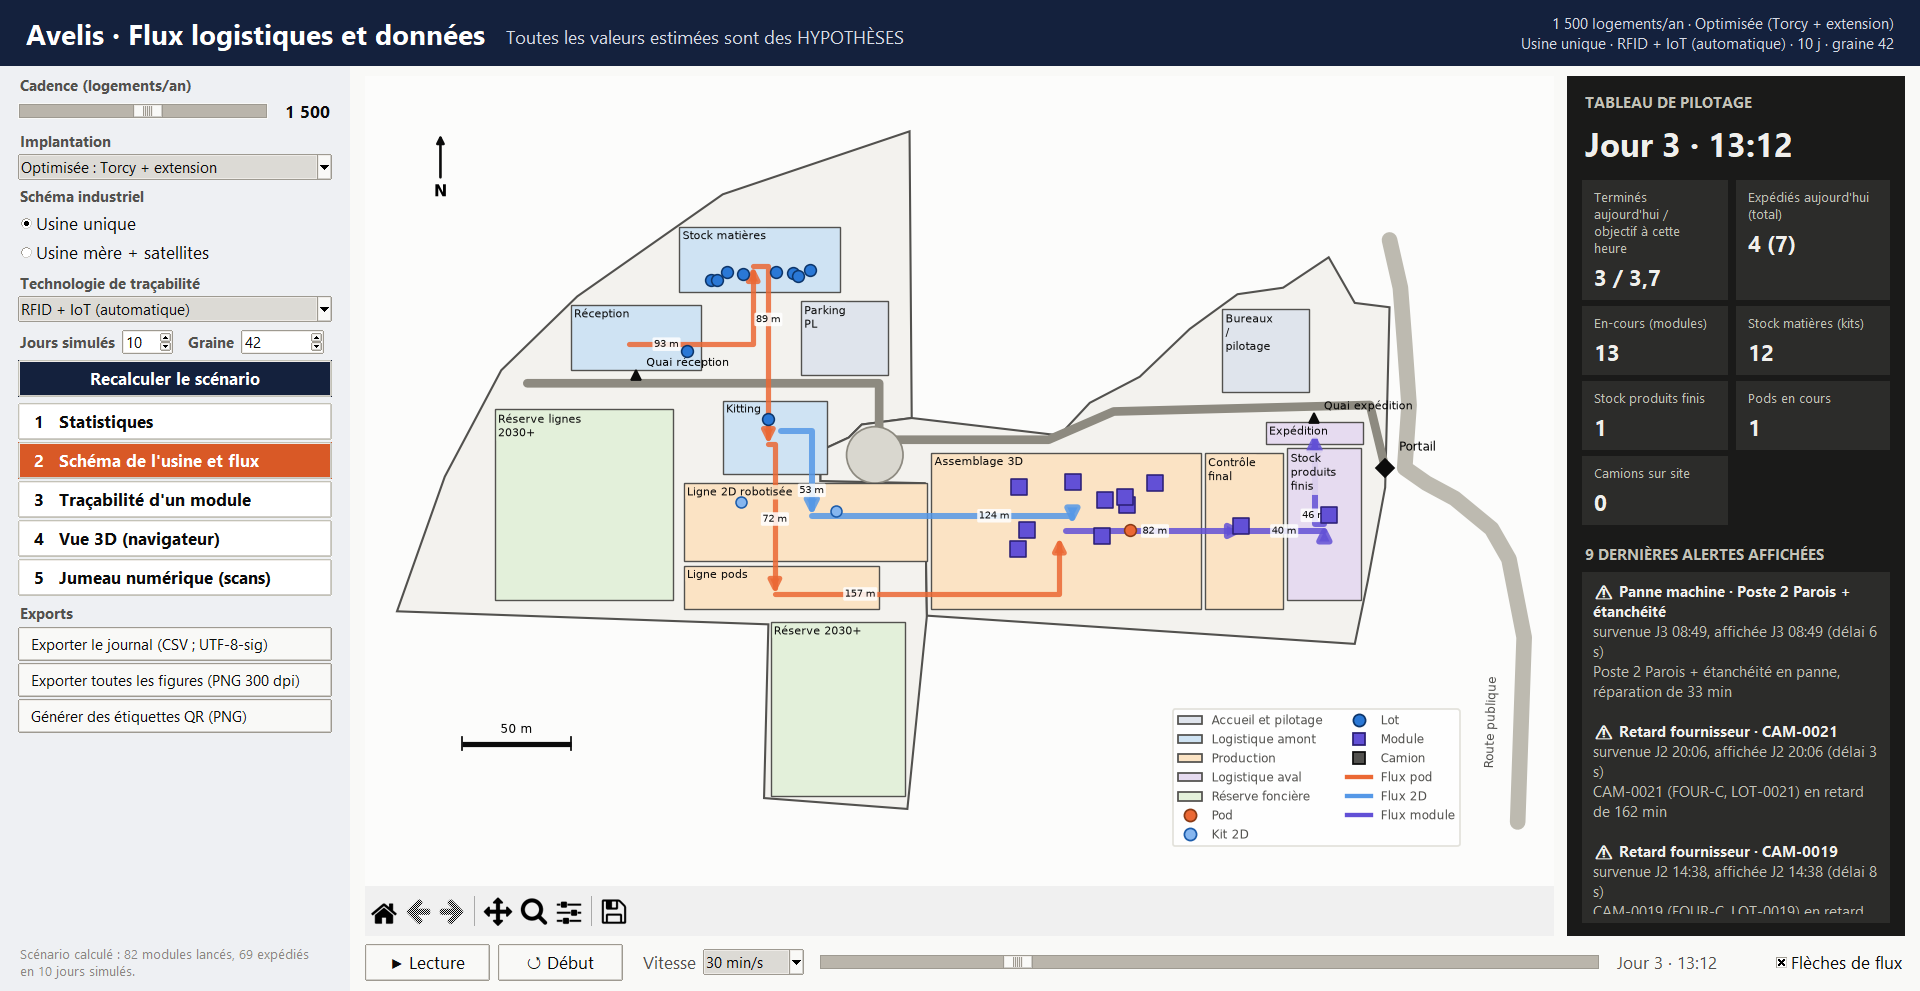
\includegraphics[width=\linewidth]{vue2_schema_optimisee.png}
\caption{Implantation optimisée animée par la SED (jour~3, 13\,h\,12). Flèches : gammes pod
(orange), 2D (bleu), module (violet), avec leurs distances. À droite, le tableau de pilotage et
les alertes horodatées (heure de l'événement et heure d'affichage).}\label{fig:schema}
\end{figure}

\paragraph{Validation par la loi de Little.} Pour l'implantation proposée, le débit
$\lambda = 8{,}125$~modules par jour de 960~min et le délai $W = 23{,}46$~h de temps d'ouverture
donnent un en-cours prédit $L = \lambda W \approx 11{,}9$~modules. La simulation mesure 11,2. L'écart
de 6\,\% correspond à la montée en charge des deux premiers jours, où l'en-cours part de zéro.
La cohérence interne du modèle est ainsi vérifiée de façon indépendante~\cite{little1961}.

\subsection{Lecture \emph{lean} de la chaîne}

Les sept gaspillages du système Toyota~\cite{ohno1988} structurent nos choix :
\begin{itemize}
\item \textbf{Transport.} L'implantation optimisée supprime 28\,\% des distances en charge et
tous les croisements ; l'expédition est placée au droit du stock de produits finis.
\item \textbf{Attente.} Le départ décalé du kit 2D synchronise murs et pod : la simulation ne
relève que 5~alertes \enquote{attente composant} sur 10~jours (82~modules lancés). Le contenu de travail de la gamme
critique (kitting, pod, assemblage, contrôle) est d'environ 22,6~h pour un délai de 23,5~h : le
rendement du processus est de l'ordre de 95\,\%. Ce chiffre est une borne haute, car le modèle
ignore les attentes administratives.
\item \textbf{Stocks.} Le stock de produits finis est dimensionné à 5~jours, soit 41~modules et
2\,148~\mdeux, mais il n'a jamais contenu plus de 4~modules en simulation, l'expédition
tirant un convoi par takt. C'est le premier levier \emph{lean} de surface : sa taille doit
devenir une décision de couverture du risque transporteur (8\,\% de retards\hyp), et non un ratio.
\item \textbf{Surproduction.} Les OF sont lancés à intervalle constant (lissage, \emph{heijunka})
et chaque module a un chantier destinataire ; le flux est tiré, pas poussé.
\item \textbf{Défauts.} Le scan refuse une étape hors séquence. C'est un détrompeur
(\emph{poka-yoke}) numérique. Un défaut déclaré bloque la pièce ; deux défauts sur un même lot, ou
une cause \enquote{matière}, bloquent tout le lot et isolent ses pièces partout (\emph{jidoka}).
\item \textbf{Mouvements inutiles.} Le kitting livre au poste exactement ce qu'il faut, et le
kanban réapprovisionne les consommables sur signal~\cite{sugimori1977}.
\item \textbf{Sur-traitement.} Les indicateurs sont calculés automatiquement à partir des
événements ; aucune ressaisie n'est nécessaire.
\end{itemize}

\subsection{Traçabilité : choix de la technologie}

\begin{figure}[!htbp]
\centering
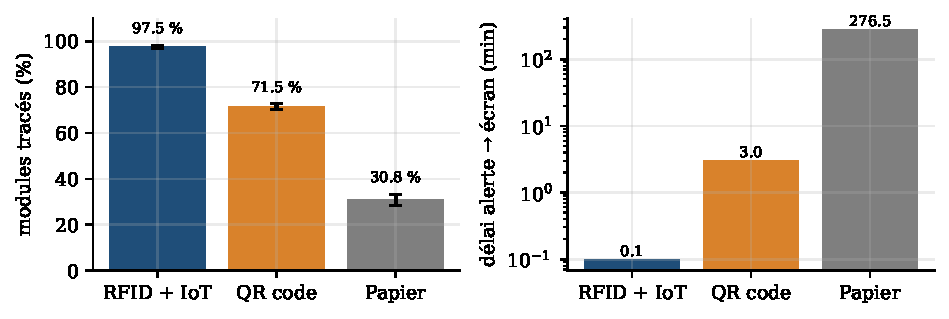
\includegraphics[width=0.85\linewidth]{tracabilite_technologies.pdf}
\caption{Part des modules expédiés tracés de bout en bout (moyenne sur 20~graines
$\pm$\,2~erreurs types) et délai moyen entre un événement et son affichage (échelle
logarithmique).}\label{fig:tracabilite}
\end{figure}

Avec une quinzaine de points obligatoires par module, l'équation~\eqref{eq:trace} est sans appel
(figure~\ref{fig:tracabilite}).
\begin{itemize}
  \item La RFID associée à l'IoT trace 97,5\,\% des modules, avec un délai d'affichage de
        quelques secondes.
  \item Le QR code scanné à la main en trace 71,5\,\%, avec 3~min de délai.
  \item Le papier n'en trace que 30,8\,\%, et l'information arrive 4,6~h après l'événement.
\end{itemize}
Les valeurs simulées encadrent les valeurs théoriques (97,3, 70,6 et 32,4\,\%), ce qui valide la
SED. Les causes de défaut ne sont retrouvées que dans 57\,\% des cas avec le papier, contre 100\,\%
avec la RFID.

Nous recommandons donc une solution hybride, cohérente avec les paliers : un marquage QR de chaque
pièce, quasi gratuit et lisible par tout opérateur, et des portiques RFID aux cinq nœuds de flux
où une lecture automatique est indispensable. Le démonstrateur, au palier~0, utilise le QR et le
téléphone.

% =============================================================================================
\section{Le jumeau numérique supervisé}\label{sec:jumeau}
% =============================================================================================

\subsection{Architecture et niveau de jumelage}

\begin{figure}[!htbp]
\centering
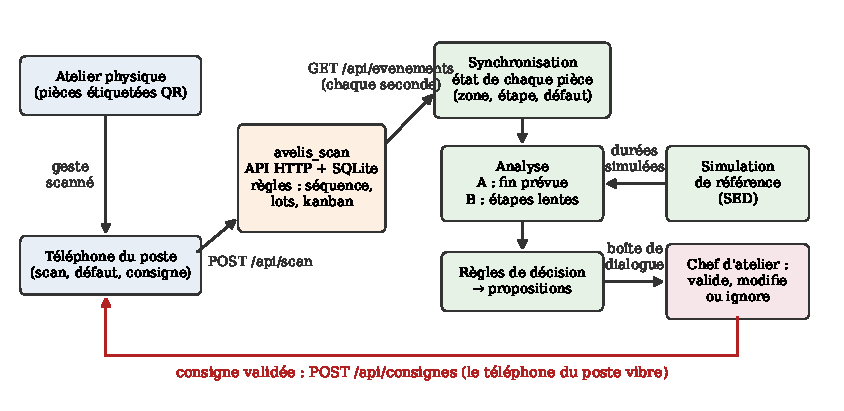
\includegraphics[width=\linewidth]{architecture_jumeau.pdf}
\caption{Boucle du jumeau. Le physique alimente le virtuel automatiquement (chaque seconde) ; le
virtuel ne revient vers le physique que par une consigne validée par un humain.}\label{fig:architecture}
\end{figure}

Chaque pièce porte un QR code qui ouvre directement sa fiche sur le téléphone du poste
(figure~\ref{fig:architecture}). Le serveur de scan applique les règles métier :
\begin{itemize}
  \item gamme imposée, refus hors séquence ;
  \item anti-double scan ;
  \item blocage des lots ;
  \item cycle kanban.
\end{itemize}
Il horodate chaque événement deux fois, à l'heure du téléphone et à l'heure du serveur. Le jumeau
interroge l'API chaque seconde, sans bloquer l'interface. Si le serveur ne répond pas, il lit
directement la base en lecture seule. Il reconstruit ainsi l'état de chaque pièce : zone du plan,
étape, défaut, lot bloqué. Les noms de zones et d'étapes sont communs au scan, à la SED et au plan,
ce qui rend la correspondance immédiate et permet d'afficher les mêmes scans sur n'importe laquelle
des trois implantations.

Dans la classification de Kritzinger et al.~\cite{kritzinger2018}, le flux physique vers virtuel
est automatique, comme dans une ombre numérique. Le flux virtuel vers physique est volontairement
\emph{semi-automatique} : le jumeau formule une consigne complète et adressée, mais elle ne part
qu'après validation. Cela correspond au niveau 5 de l'échelle de Parasuraman et
al.~\cite{parasuraman2000}, où la machine propose et exécute si l'humain approuve. Nous parlons
de \textbf{jumeau à boucle supervisée}. Ce choix n'est pas une limite technique : il découle des
verrous V5 et de l'Industrie~5.0. Il transpose aussi le \emph{jidoka} au numérique : le système
détecte et signale, l'humain décide et résout.

\begin{figure}[!htbp]
\centering
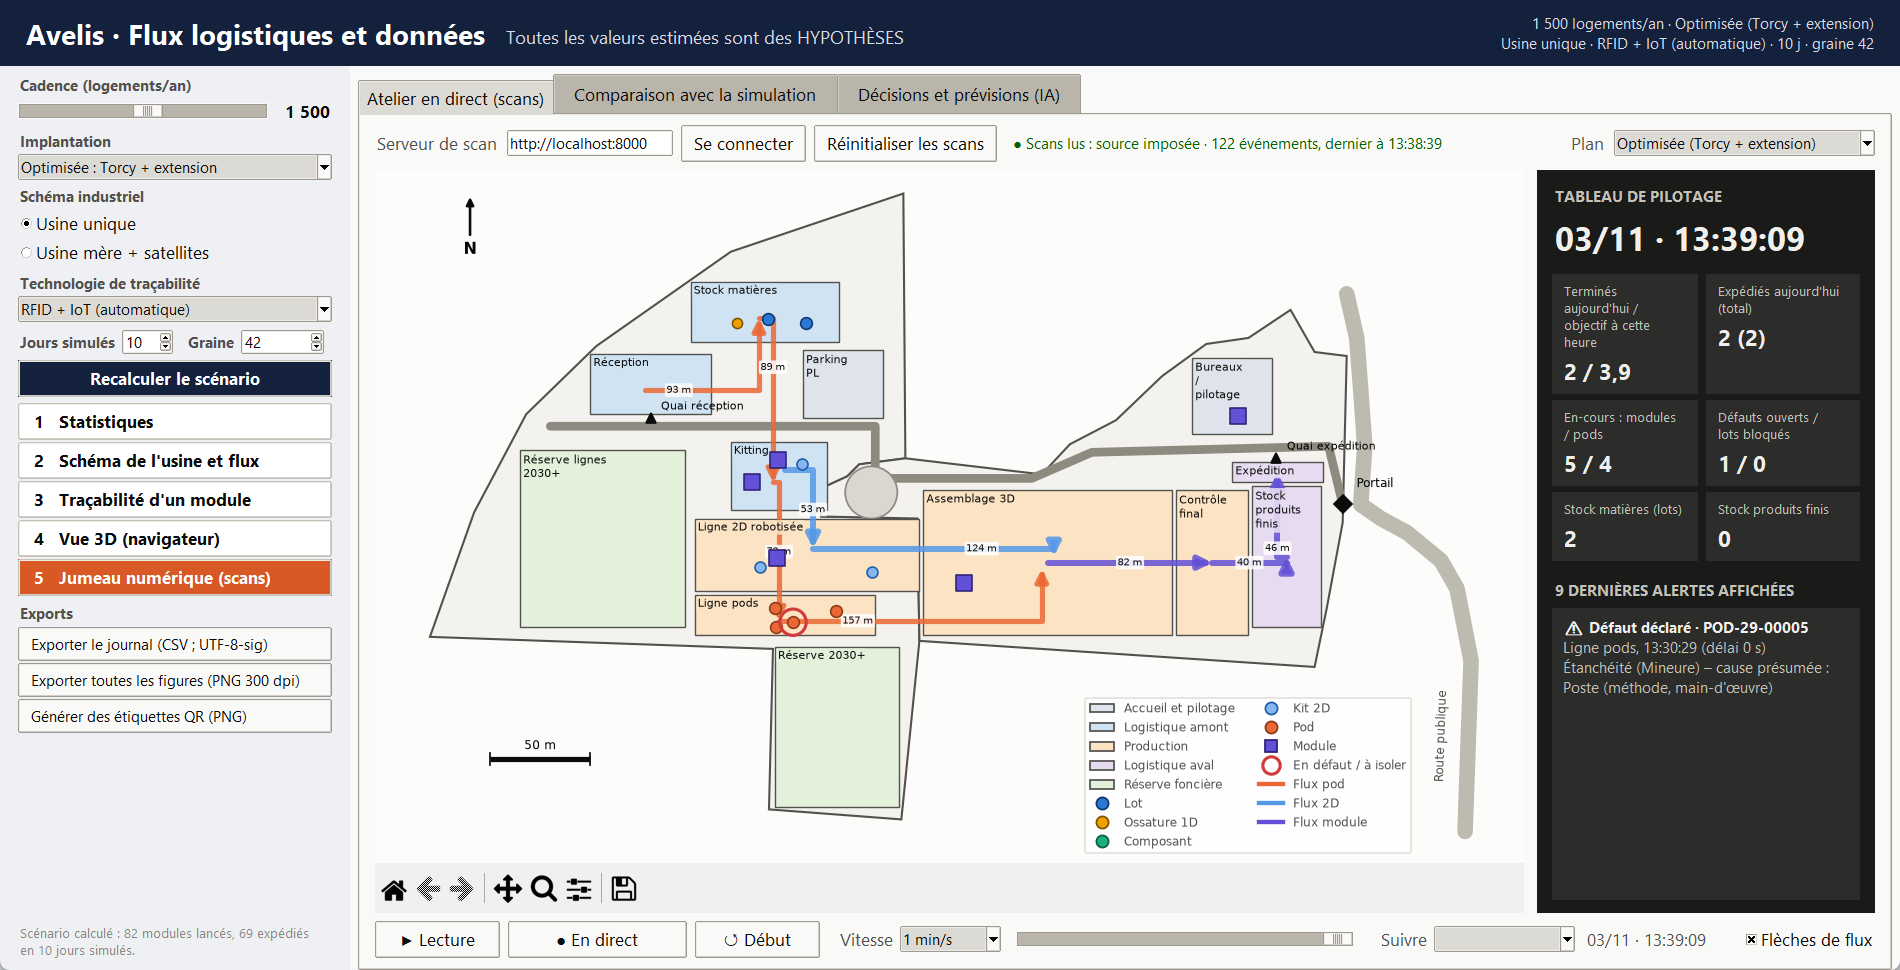
\includegraphics[width=\linewidth]{vue5_direct.png}
\caption{Onglet \enquote{Atelier en direct (scans)} sur l'implantation optimisée : sept modules à
divers stades, un pod en défaut au poste~2 (anneau rouge), tableau de pilotage à l'heure réelle et
alerte avec son délai d'enregistrement.}\label{fig:direct}
\end{figure}

\subsection{Comparaison avec la simulation}

Le jumeau compare en continu le réel à la SED de la même usine (même plan, même cadence, même
graine) :
\begin{itemize}
  \item sur six indicateurs : délai OF $\rightarrow$ stock PF, débit, défauts par module, délai
        d'affichage, part tracée, scans refusés ;
  \item sur la durée de chaque étape des gammes module et pod (figure~\ref{fig:comparaison}).
\end{itemize}
Une étape est qualifiée \enquote{plus lente} ou \enquote{plus rapide} au-delà de 50\,\% d'écart\hyp.
Sur la maquette, un geste dure quelques minutes au lieu de plusieurs heures. Toutes les étapes
apparaissent donc \enquote{plus rapides} (rapport 0,01 à 0,65), ce qui illustre la nécessité
d'un facteur d'échelle de temps explicite (\code{echelle\_temps\_maquette}\hyp). C'est un point de
méthode important : un jumeau ne vaut que par le recalage de son modèle.

\begin{figure}[!htbp]
\centering
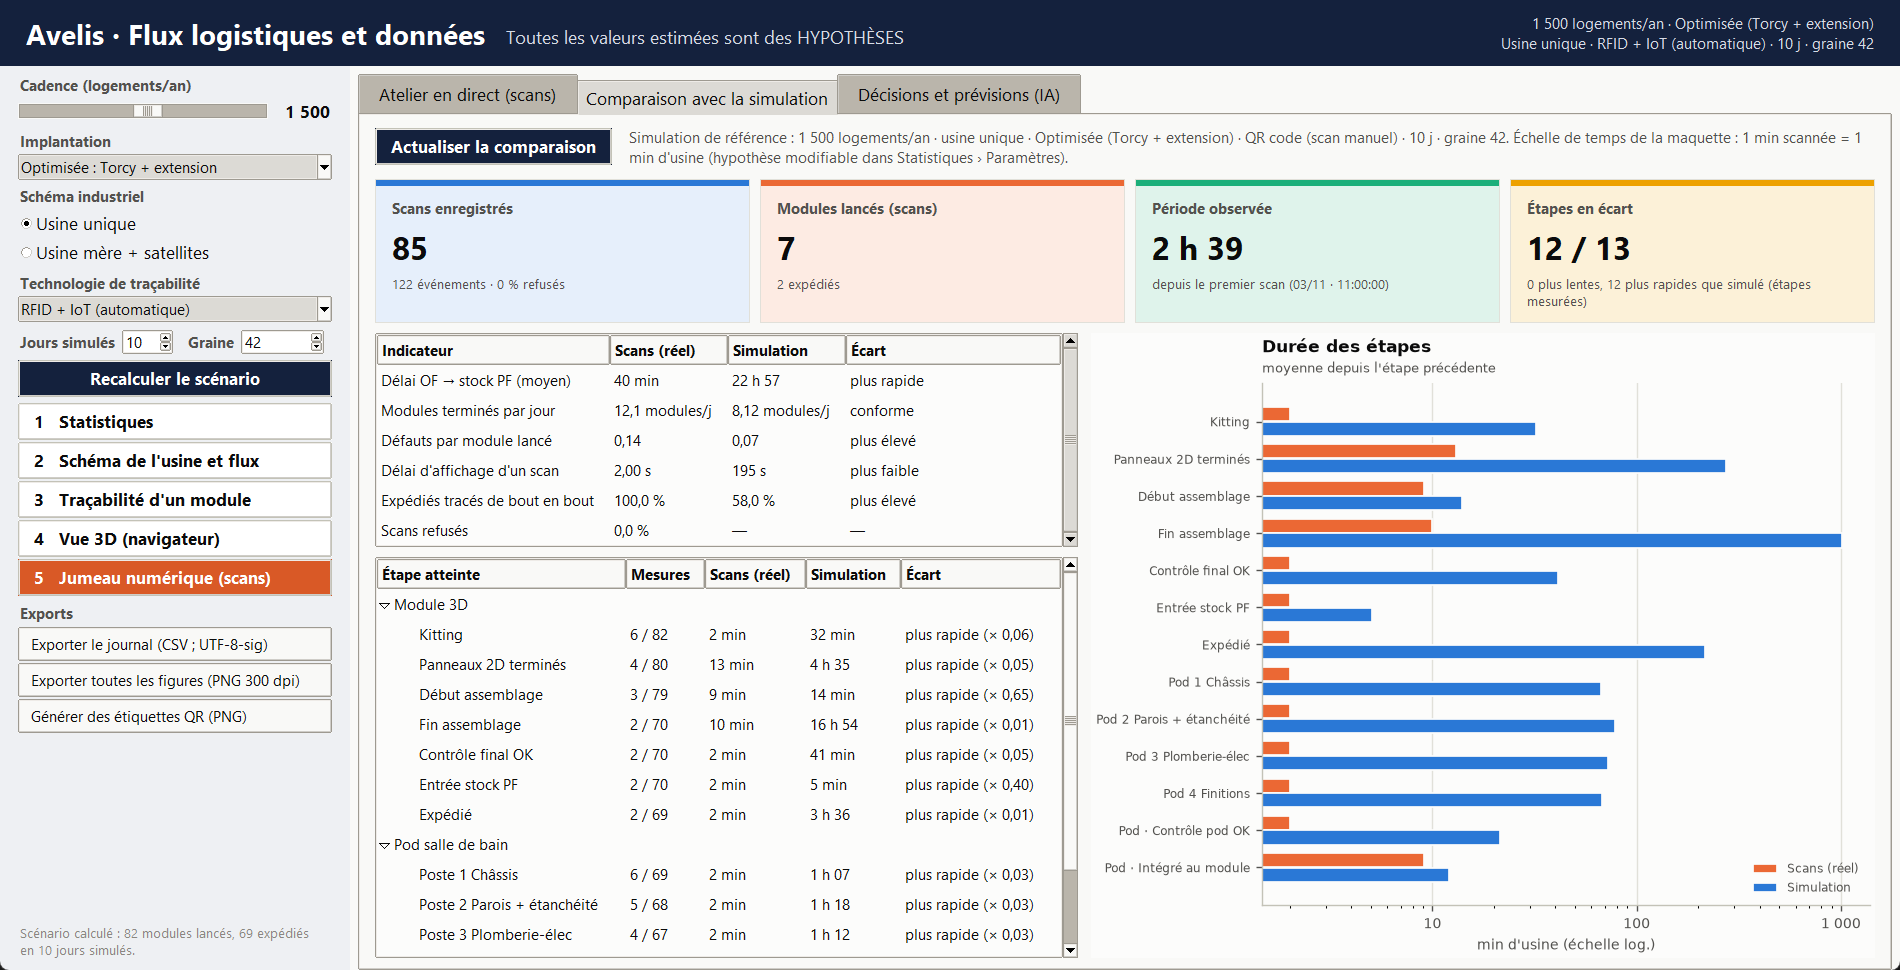
\includegraphics[width=\linewidth]{vue5_comparaison.png}
\caption{Comparaison du réel (scans de la maquette) avec la simulation de référence : indicateurs,
durée de chaque étape et graphique en échelle logarithmique.}\label{fig:comparaison}
\end{figure}

\subsection{Option A : prévision des fins de fabrication}

Pour un module en cours, à l'étape $e_0$ atteinte à l'instant $t_0$, la fin de fabrication prévue
est la somme des durées estimées des transitions restantes $\mathcal{R}$. Chaque durée est un
estimateur de crédibilité~\cite{buhlmann1967} : la moyenne $\bar{x}_e$ de $n_e$ mesures est
rapprochée de la durée simulée $\mu^{\text{sim}}_e$ avec un poids $k = 5$\hyp,
\begin{equation}\label{eq:credibilite}
\hat{\mu}_e = \frac{n_e\,\bar{x}_e + k\,\mu^{\text{sim}}_e}{n_e + k}, \qquad
\hat{T} = t_0 + \sum_{e \in \mathcal{R}} \hat{\mu}_e, \qquad
\hat{T}_{10/90} = \hat{T} \mp z_{0{,}9}\Big(\sum_{e\in\mathcal{R}} \hat{\sigma}_e^2\Big)^{1/2},
\end{equation}
avec $z_{0{,}9} = 1{,}2816$. Au démarrage ($n_e = 0$), la prévision est celle de la simulation ;
avec l'expérience, elle converge vers les mesures. C'est exactement le comportement voulu quand
les données sont rares (V5).

La prévision est évaluée hors échantillon sur la SED de référence (1\,500 logements/an, 10~jours,
graine~42) :
\begin{itemize}
  \item elle apprend sur la première moitié des modules terminés ;
  \item elle prévoit, à chaque étape de la seconde moitié, la fin de fabrication ;
  \item l'erreur obtenue est comparée à la référence naïve \enquote{OF + délai moyen}~\cite{hyndman2021}.
\end{itemize}
Sur 216~prévisions et 36~modules, l'erreur absolue moyenne est de \textbf{52,9~min contre
79,8~min} pour la référence naïve, soit 34\,\% de moins. L'ordre de grandeur est utile pour un délai
moyen de 23~h : il suffit pour prévenir l'expédition et le transporteur d'un retard dans la
journée.

\subsection{Option B : détection des étapes anormalement lentes}

Pour chaque étape, la référence est la médiane $\tilde{x}$ des passages antérieurs, ou la durée
simulée tant qu'il y a moins de 3~passages. La dispersion est mesurée par l'écart absolu médian
normalisé, $s = 1{,}4826\,\mathrm{MAD}$, avec un plancher de 10\,\% de la médiane. On compare la
moyenne $\bar{x}_{(3)}$ des trois derniers passages à cette référence :
\begin{equation}\label{eq:optionb}
r = \frac{\bar{x}_{(3)}}{\tilde{x}}, \qquad
\text{anormal si } r > 1{,}5 ; \qquad
\text{à surveiller si } r > 1{,}25 \text{ ou } \max x_{(3)} > \tilde{x} + 3s .
\end{equation}

La médiane et le MAD résistent aux valeurs aberrantes, contrairement à la moyenne et à
l'écart-type~\cite{rousseeuw1993,leys2013}. Une pause ou un double scan ne masque donc pas une
dérive réelle.

Sur un atelier de scan où le poste~2 de la ligne pods passe de 2 à 10~min à partir du sixième
pod, la dérive est classée \enquote{anormale} ($r = 5{,}0$) dès le troisième passage lent. Les
autres postes restent normaux ($r = 1{,}0$) : il n'y a aucune fausse alarme
(figure~\ref{fig:optionb}).

\begin{figure}[!htbp]
\centering
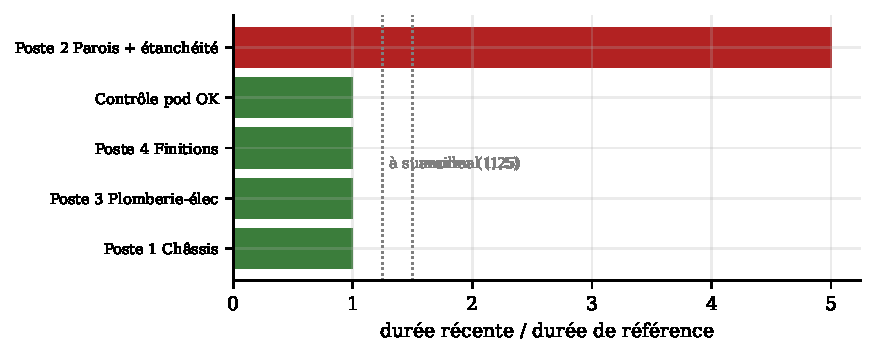
\includegraphics[width=0.74\linewidth]{option_b_postes.pdf}
\caption{Option B sur un atelier dont le poste~2 de la ligne pods est ralenti : rapport entre la
durée récente et la référence, par étape.}\label{fig:optionb}
\end{figure}

\subsection{Décisions proposées, humain dans la boucle}

Quatre règles explicites transforment l'analyse en propositions. Tous leurs seuils sont des
hypothèses modifiables :
\begin{enumerate}
  \item \textbf{Étape anormalement lente} (option B) : une consigne est adressée au poste et au
        bureau.
  \item \textbf{Pièces bloquées} : une pièce n'a pas été scannée depuis plus de 2~fois la durée
        estimée de l'étape suivante, dans la journée. Les pièces sont regroupées par poste et par
        étape, pour éviter une rafale de dialogues.
  \item \textbf{Défauts répétés} : 2~défauts de même catégorie au même poste en 60~min.
  \item \textbf{Retard sur l'objectif du jour} : moins de 80\,\% de l'objectif à cette heure.
\end{enumerate}
Chaque proposition ouvre une boîte de dialogue (figure~\ref{fig:dialogue}). Elle indique la règle,
le motif chiffré, les destinataires et une consigne \emph{modifiable}. L'opérateur peut l'envoyer,
l'ignorer ou décider plus tard. Une décision traitée n'est pas reproposée avant 60~min, et aucune
consigne ne part sans validation. L'historique des décisions, avec leur statut, constitue une
trace d'audit de la décision humaine.

\begin{figure}[!htbp]
\centering
\begin{subfigure}[b]{0.36\linewidth}\centering
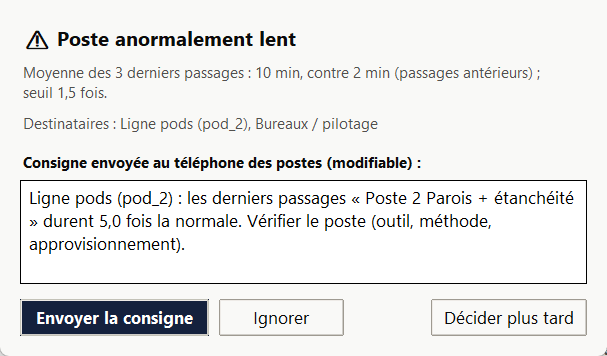
\includegraphics[width=\linewidth]{dialogue_decision.png}
\caption{Proposition soumise à l'humain.}
\end{subfigure}\hfill
\begin{subfigure}[b]{0.62\linewidth}\centering
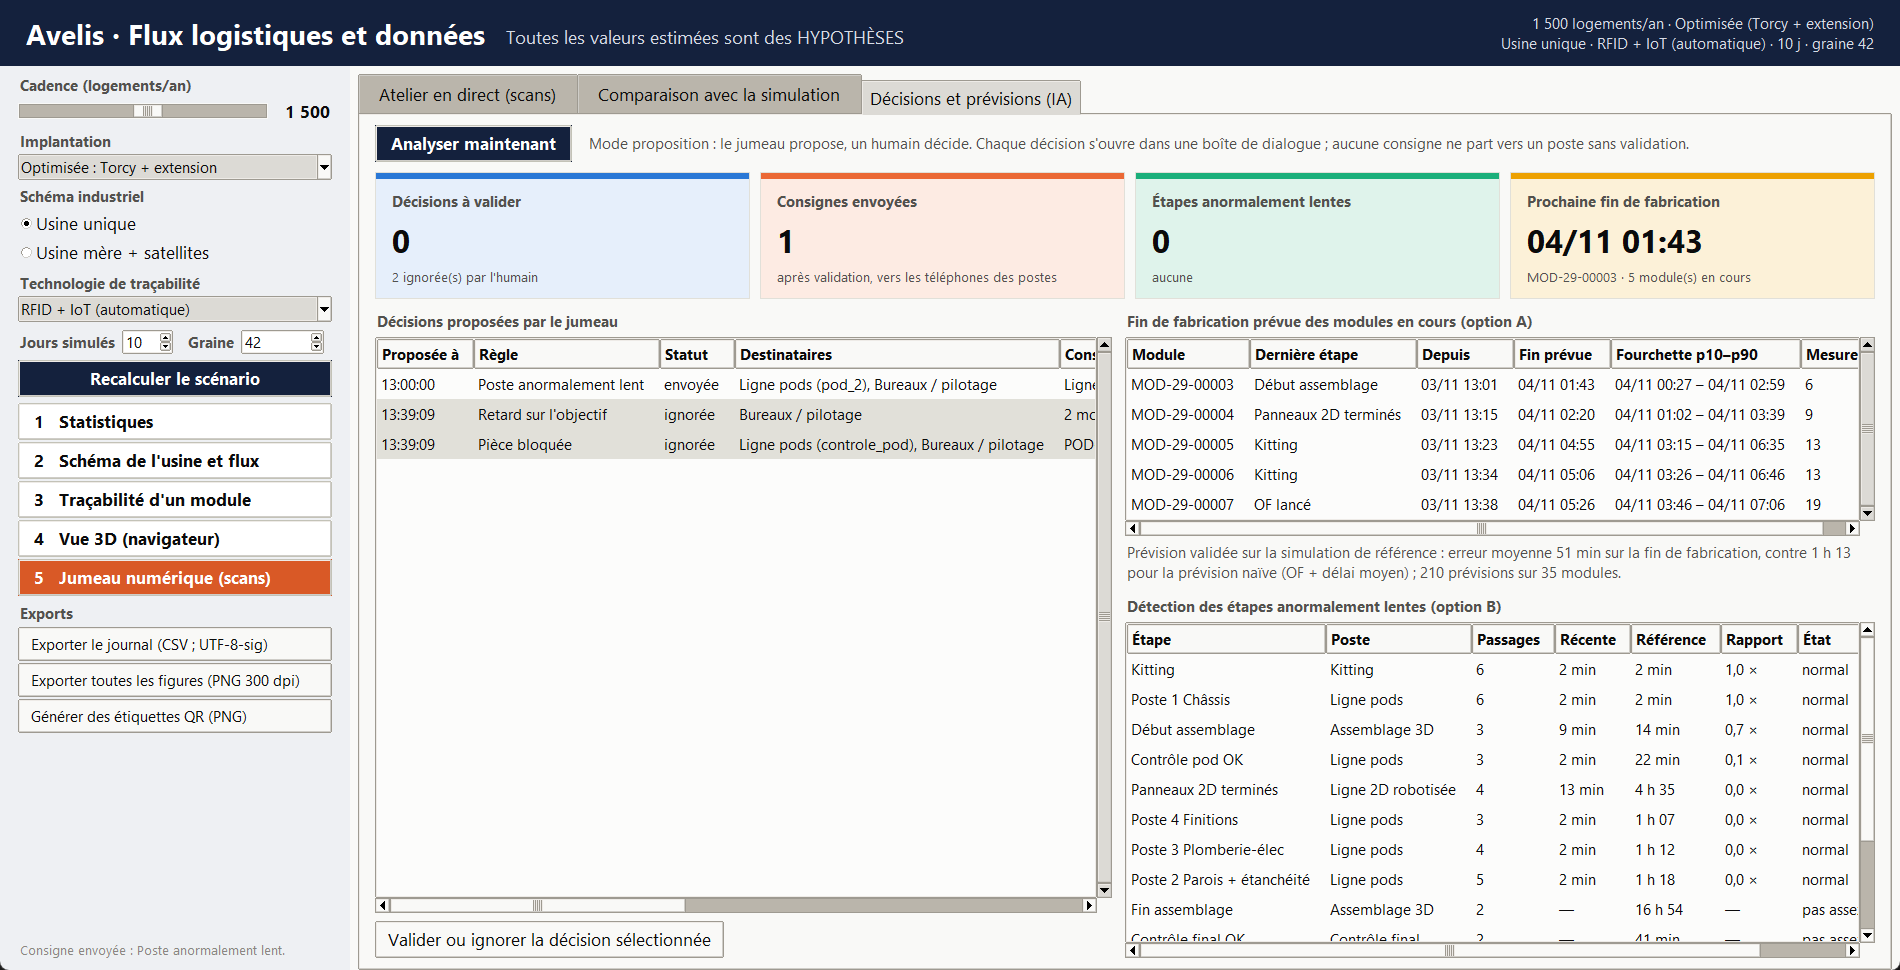
\includegraphics[width=\linewidth]{vue5_decisions.png}
\caption{Historique, prévisions (option A) et étapes (option B).}
\end{subfigure}
\caption{Onglet \enquote{Décisions et prévisions (IA)} du jumeau.}\label{fig:dialogue}
\end{figure}

\subsection{Pourquoi cette solution ? Comparaison avec les alternatives}

\begin{table}[!htbp]
\centering\footnotesize
\caption{Alternatives envisagées pour le pilotage des flux (++ très favorable, -- très
défavorable).}\label{tab:alternatives}
\begin{tabularx}{\linewidth}{@{}lYYYYY@{}}
\toprule
Critère & Management visuel seul (andon, tableaux) & Progiciel MES / ERP du marché &
Simulation hors ligne seule & Jumeau autonome (apprentissage profond) & \textbf{Jumeau supervisé
(retenu)} \\
\midrule
État réel synchronisé & -- (manuel) & ++ & -- & ++ & + (1~s) \\
Traçabilité par composant & -- & ++ & -- & + & ++ \\
Prévision, détection & -- & + & -- (hors ligne) & ++ (si données) & + (mesurée) \\
Données nécessaires & ++ & + & ++ & -- (massives) & ++ (quelques passages) \\
Explicabilité & ++ & -- (boîte noire) & + & -- & ++ (règles, crédibilité) \\
Place de l'humain & ++ & + & + & -- (hors boucle) & ++ (valide tout) \\
Coût, délai, palier~0 & ++ & -- & + & -- & ++ \\
\bottomrule
\end{tabularx}
\end{table}

Le tableau~\ref{tab:alternatives} résume l'arbitrage entre les cinq options.
\begin{itemize}
  \item \textbf{Le management visuel} est l'âme du \emph{lean}, mais il ne trace pas les composants
        et n'anticipe rien. Notre jumeau le prolonge, puisque ses tuiles sont celles d'une revue de
        performance quotidienne ; il ne le remplace pas.
  \item \textbf{Un progiciel MES} offre une couverture fonctionnelle supérieure. Il suppose
        toutefois des processus stabilisés et un coût d'intégration incompatible avec le
        palier~0, et ses algorithmes restent opaques.
  \item \textbf{La simulation seule} dimensionne mais ne voit pas le réel. Nous la conservons comme
        référence du jumeau.
  \item \textbf{Un jumeau autonome} à apprentissage profond exigerait des milliers d'exemples que
        l'usine ne produira pas avant des années. Il retirerait aussi l'humain de la boucle, avec
        les risques décrits par Bainbridge~\cite{bainbridge1983}, à rebours de
        l'Industrie~5.0~\cite{breque2021}.
\end{itemize}
Le jumeau supervisé est la seule option qui soit, dès le palier~0, synchronisée, traçable,
explicable, frugale en données et centrée sur l'humain. Il peut ensuite migrer vers un MES quand
les processus seront stabilisés : ses données et son API sont ouvertes.

% =============================================================================================
\section{Cas d'application}\label{sec:cas}
% =============================================================================================

\subsection{Cas 1 : hébergement des salariés des grands chantiers nucléaires (Gravelines et
Flamanville)}

\paragraph{Contexte et dimensionnement du besoin.} Les grands chantiers électronucléaires
concentrent pendant plusieurs années des milliers de salariés loin des bassins de logement.
\begin{itemize}
  \item À \textbf{Gravelines} (Nord), le projet de deux réacteurs EPR2 mobilisera au moins 8\,000
        salariés au pic. L'hypothèse de travail des services de l'État est que la moitié devra être
        logée à proximité~\cite{prefgravelines}.
  \item À \textbf{Penly}, chantier comparable, 6\,000 places d'hébergement sont prévues à moins de
        30~km, dont 4\,000 en logements modulables~\cite{prefpenly}.
  \item À \textbf{Flamanville} (Manche), le chantier de l'EPR a conduit à héberger 12\,500 salariés
        en cumul, notamment dans des mobil-homes~\cite{aieflamanville}. Ce retour d'expérience
        montre l'enjeu de qualité d'un hébergement de chantier pérenne.
\end{itemize}
En transposant à Gravelines la part modulaire de Penly (deux tiers), le besoin modulaire est
d'environ 2\,700~logements\hyp{} ; nous y ajoutons un besoin résiduel à Flamanville. Le
scénario retenu est un programme de 1\,200~logements par an\hyp{} pendant trois ans, réparti à
70\,\% vers Gravelines et 30\,\% vers Flamanville\hyp. Ce programme est compatible avec la capacité
de Torcy.

Les logements T1 et T1~bis d'Avelis correspondent à ce besoin de logement individuel de longue
durée. Le caractère démontable des modules ouvre une seconde vie après le pic du chantier :
logement étudiant, logement social ou relogement. C'est la logique \enquote{d'héritage} du grand
chantier et de réutilisation identifiée par la littérature~\cite{kamali2016}.

\paragraph{Contrainte de transport.} Gravelines est à 650~km de route de Torcy et Flamanville à
730~km\hyp. Un module de 3,5~m de large voyage en convoi exceptionnel de deuxième
catégorie~\cite{arrete2006} : 11,2~h de trajet moyen à 60~km/h\hyp, soit plus d'une journée de
circulation autorisée et un retour à vide. Un kit de murs et de pod, lui, voyage en semi-remorque
standard, à trois kits par camion.

\begin{figure}[!htbp]
\centering
\begin{subfigure}[b]{0.40\linewidth}\centering
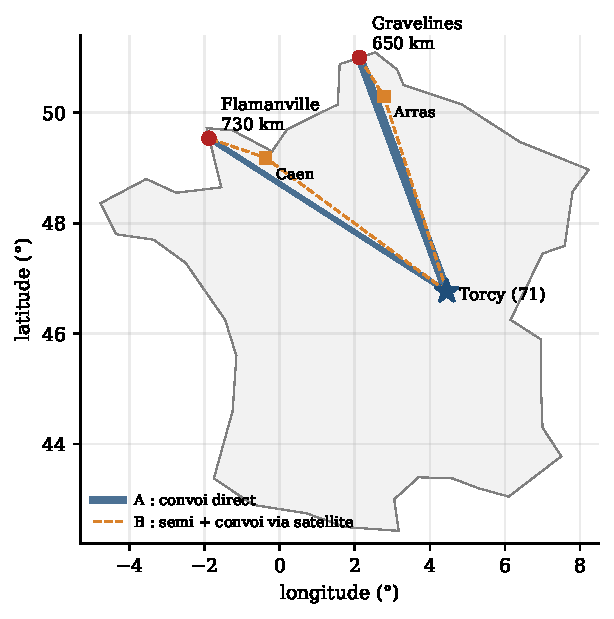
\includegraphics[width=\linewidth]{carte_nucleaire.pdf}
\caption{Itinéraires A et B.}
\end{subfigure}\hfill
\begin{subfigure}[b]{0.58\linewidth}\centering
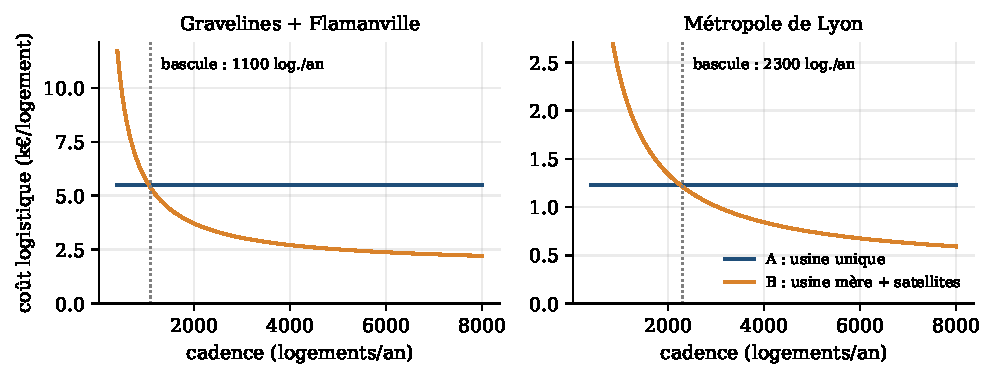
\includegraphics[width=\linewidth]{sensibilite_reseaux.pdf}
\caption{Coût logistique par logement selon la cadence.}
\end{subfigure}
\caption{Cas d'application. (a)~Livraison directe depuis Torcy (A) ou via une unité d'assemblage
(B). (b)~Le point de bascule est de 1\,100 logements/an pour les chantiers nucléaires, contre
2\,300 pour la seule métropole de Lyon.}\label{fig:reseaux}
\end{figure}

\begin{table}[!htbp]
\centering\small
\caption{Bilans logistiques annuels des réseaux. A : usine unique ; B : usine mère et unités
d'assemblage. Modèle de l'équation~\eqref{eq:reseau}.}\label{tab:reseaux}
\begin{tabularx}{\linewidth}{@{}Yrrrrr@{}}
\toprule
Cas (cadence) & Coût (\EUR/logement) & \COdeux{} (t/an) & Délai moyen (h) & Distance (km) & Bascule (log./an) \\
\midrule
\multicolumn{6}{@{}l}{\textit{Cas 1 : Gravelines 70\,\% + Flamanville 30\,\% (1\,200 log./an)}} \\
A : convois directs depuis Torcy & 5\,501 & 1\,942 & 11,2 & 674 & --- \\
B : unités à Arras et Caen & 5\,047 & 791 & 9,5 & 677 & 1\,100 \\
B : unités foraines à Dunkerque et Cherbourg & \textbf{4\,348} & \textbf{585} & 9,3 & 693 & \textbf{900} \\
\midrule
\multicolumn{6}{@{}l}{\textit{Cas 2 : métropole de Lyon (300 log./an)}} \\
A : convois directs depuis Torcy & \textbf{1\,230} & \textbf{108} & 2,5 & 151 & --- \\
B : unité à Lyon-Sud & 7\,009 & 44 & 2,5 & 185 & 2\,300 \\
\midrule
\multicolumn{6}{@{}l}{\textit{Référence : demande nationale diffuse, 8~métropoles (1\,500 log./an)}} \\
A : usine unique & \textbf{3\,083} & 1\,360 & 6,3 & 378 & --- \\
B : trois satellites (variante \enquote{hybride}) & 5\,606 & 813 & 6,0 & 408 & 4\,100 \\
\bottomrule
\end{tabularx}
\end{table}

\paragraph{Résultat.} Pour ce programme lointain et concentré, le schéma s'inverse
(tableau~\ref{tab:reseaux}, figure~\ref{fig:reseaux}). Des unités d'assemblage foraines au plus
près des chantiers (Dunkerque, Cherbourg) réduisent le coût logistique par logement de 21\,\% et
les émissions de transport de 70\,\% (585 contre 1\,942~t de \COdeux{} par an). Elles suppriment
aussi le transport exceptionnel sur longue distance et rendent la livraison indépendante des
fenêtres de circulation des convois. Le point de bascule tombe à 900~logements par an.

Le résultat est robuste à l'hypothèse la plus défavorable aux unités foraines : amorties sur
8~ans de programme au lieu de 15, elles coûtent 2,5~M\EUR{} par an chacune et le coût par logement
reste inférieur à celui de l'option A (5\,223 contre 5\,501\EUR).

L'organisation qui en découle est la suivante : Torcy reste l'usine unique pour la demande
diffuse et devient \emph{usine mère} pour le programme nucléaire, en y consolidant murs et pods en
kits. L'assemblage 3D est déporté dans des unités temporaires, démontées en fin de programme.
L'implantation optimisée s'y prête : la halle d'assemblage libérée par ce programme absorbe la
croissance de la demande diffuse.

\paragraph{Ce que le jumeau apporte à ce cas.} Avec deux sites d'assemblage distants, la
prévision de fin de fabrication (option A) devient une prévision de départ des semi-remorques.
La traçabilité par composant suit le kit de Torcy jusqu'au logement monté. Les règles
\enquote{pièces bloquées} et \enquote{retard sur l'objectif} s'appliquent à chaque unité
foraine, avec un chef d'atelier local dans la boucle. La capture de l'onglet \enquote{Réseau} du
logiciel paramétré pour ce cas figure en annexe~\ref{ann:captures}.

\subsection{Cas 2 : programme urbain dans la métropole de Lyon}

Le second cas est un programme classique de 300~logements par an dans la métropole de Lyon,
à 151~km de route de Torcy. La livraison directe en convoi prend 2,5~h et coûte 1\,230\EUR{} par
logement. Une unité d'assemblage locale ne deviendrait rentable qu'au-delà de 2\,300~logements par
an, car ses coûts fixes ne sont pas compensés par l'économie de transport sur une distance aussi
courte. \textbf{L'usine unique s'impose}, et la proximité de Torcy avec le couloir rhodanien est un
atout de localisation.

\paragraph{Synthèse.} Le bon schéma industriel n'est pas une propriété de l'usine mais du couple
(usine, demande). Il dépend de la distance pondérée et de la concentration de la demande :
\begin{itemize}
  \item pour une demande diffuse ou proche (Lyon, réseau national), l'usine unique à Torcy est
        optimale jusqu'à plus de 4\,000~logements par an ;
  \item pour un grand programme lointain et concentré (chantiers nucléaires), des unités foraines
        deviennent préférables dès 900~logements par an.
\end{itemize}
Le modèle de réseau intégré au logiciel permet d'instruire ce choix contrat par contrat.

% =============================================================================================
\section{Discussion et limites}\label{sec:discussion}
% =============================================================================================

\begin{itemize}
\item \textbf{Données.} Presque tous les paramètres sont des hypothèses : temps de cycle, taux de
défaut, coûts kilométriques, coûts fixes des satellites. Les conclusions structurelles résistent
aux variations raisonnables. C'est le cas du goulot d'assemblage, du débit indépendant de
l'implantation et du rôle de la géographie de la demande, que montrent les courbes de sensibilité.
Les valeurs absolues, elles, devront être recalées dès que le palier~0 produira des mesures.
Le jumeau est précisément l'outil de ce recalage.
\item \textbf{Écarts aux ordres de grandeur attendus.} Le takt calculé (93,9~min) diffère de
l'ordre de grandeur de 90~min, parce que nous avons retenu les 220~jours ouvrés communs aux
blocs. Le schéma satellites dépasse légèrement l'objectif simulé (100,8\,\%), car la
consolidation est plus courte que l'assemblage. Ces écarts sont expliqués, sans ajustement des
hypothèses.
\item \textbf{Implantation.} L'implantation optimisée repose sur des zones rectangulaires et des
distances de centre à centre. Elle est meilleure que les alternatives, mais pas prouvée optimale.
Une résolution exacte ou métaheuristique du problème d'implantation~\cite{drira2007} sur le
contour réel est une suite naturelle.
\item \textbf{Jumeau.} La validation de l'option A est faite sur la simulation, pas encore sur des
données réelles d'Avelis. La maquette montre la chaîne complète, du scan à la consigne, mais
avec des durées de démonstration.
\item \textbf{Hors périmètre.} La gouvernance des données et la cybersécurité de l'API (IEC
62443~\cite{iec62443}) sont à traiter avant tout déploiement.
\end{itemize}

% =============================================================================================
\section{Conclusion}
% =============================================================================================

Nous avons traité la chaîne d'Avelis comme un système de flux unique. Le dimensionnement fixe le
takt à 93,9~min et désigne l'assemblage 3D comme goulot. L'implantation optimisée sur le foncier
de Torcy agrandi supprime 28\,\% des distances en charge et tous les croisements, sans toucher au
débit, ce que la théorie des contraintes et la loi de Little expliquent. La traçabilité par
composant impose une lecture automatique aux nœuds de flux.

Le jumeau numérique supervisé, alimenté par le scan réel des pièces, synchronise le plan chaque
seconde et compare le réel à la simulation. Il prévoit les fins de fabrication avec 34\,\%
d'erreur en moins qu'une référence naïve et isole un poste ralenti sans fausse alarme. Il propose
des consignes que seul l'humain valide : c'est notre réponse à la question du défi, placer
l'humain au bon endroit, c'est-à-dire au point de décision, éclairé par les données.

Enfin, les deux cas d'application montrent que le schéma industriel doit se décider contrat par
contrat. L'usine unique reste la règle, et des unités foraines deviennent l'exception rentable et
sobre pour les grands programmes lointains, comme l'hébergement des chantiers nucléaires de
Gravelines et de Flamanville.

\printbibliography[heading=bibintoc,title={Références}]

% =============================================================================================
\appendix
\section{Hypothèses principales}\label{ann:hypotheses}
% =============================================================================================

\begin{table}[!htbp]
\centering\small
\caption{Principales valeurs du modèle (A : donnée Avelis ; H : hypothèse de l'équipe, modifiable
dans l'onglet \enquote{Paramètres}).}
\begin{tabularx}{\linewidth}{@{}Yrl@{}}
\toprule
Paramètre & Valeur & Statut \\
\midrule
Cadence cible (haut de la fourchette) & 1\,500 logements/an & A \\
Emprise actuelle / extension & 42\,786 / 27\,443~\mdeux & A \\
Modules / pods par logement & 1,2 / 1,0 & H \\
Jours ouvrés, équipes & 220~j, 2\,$\times$\,8~h & H (commun aux blocs) \\
TRS, charge maximale d'une ressource & 0,80 ; 0,90 & H \\
Travail d'assemblage 3D par module & 960~min & H \\
Cycle ligne 2D ; postes pods & 70~min ; 60 / 75 / 70 / 65~min & H \\
Matières par logement, charge utile d'un camion & 12~t ; 14~t & H \\
Couverture stock matières / produits finis & 10~j / 5~j & H \\
Retards fournisseurs / transporteurs ; lots non conformes & 12\,\% / 8\,\% ; 6\,\% & H \\
Gabarit d'un module & 3,5\,$\times$\,10\,$\times$\,3,2~m & H \\
Coût kilométrique convoi / semi ; \COdeux & 3,4 / 1,9\EUR/km ; 1~kg/km & H \\
Satellite : investissement, amortissement, frais fixes & 9~M\EUR, 15~ans, 1,4~M\EUR/an & H \\
Jumeau : poids de la prévision $k$ ; seuils de l'option B & 5 ; 1,25 / 1,5 / 3~MAD & H \\
Cas 1 : cadence, parts de la demande & 1\,200~log./an ; 70\,\% / 30\,\% & H (scénario) \\
\bottomrule
\end{tabularx}
\end{table}

\section{Captures complémentaires du logiciel}\label{ann:captures}

\begin{figure}[!htbp]
\centering
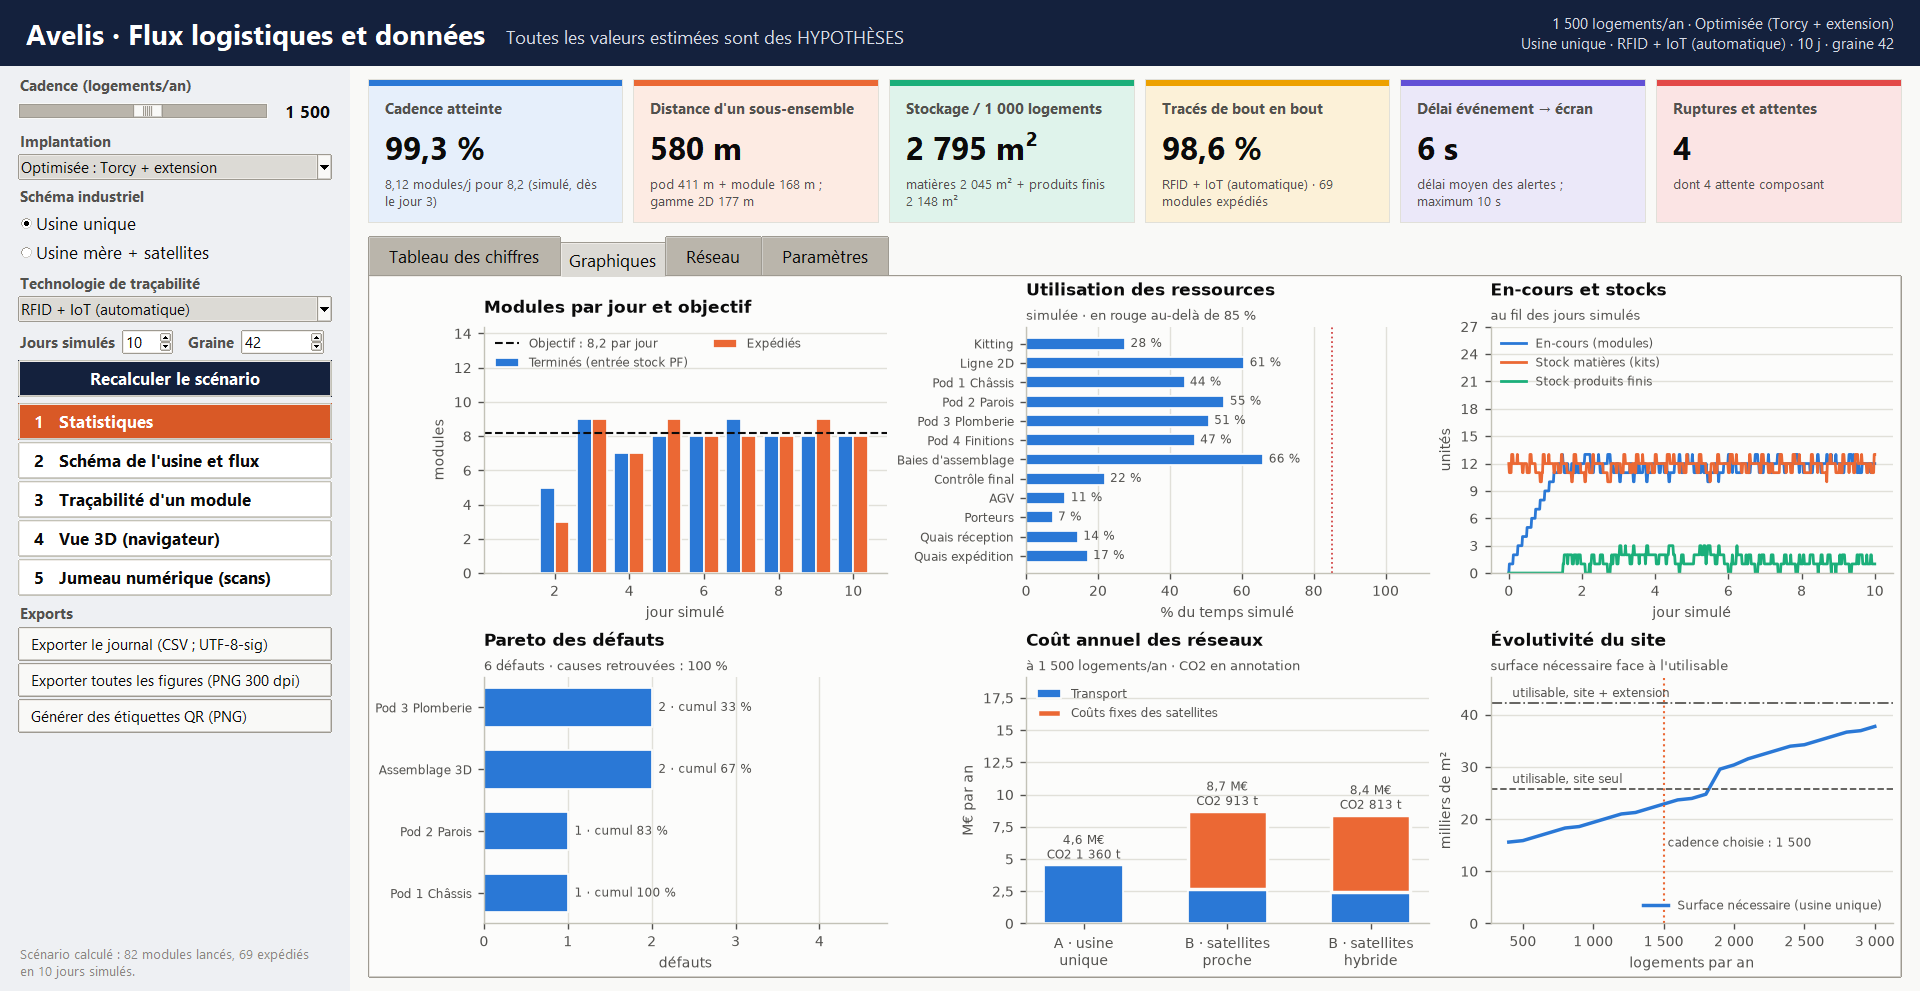
\includegraphics[width=\linewidth]{vue1_graphiques.png}
\caption{Vue \enquote{Statistiques}, onglet \enquote{Graphiques} (implantation optimisée,
1\,500 logements/an) : débit journalier, utilisation des ressources, en-cours et stocks, Pareto
des défauts, coût annuel des réseaux, évolutivité du site.}
\end{figure}

\begin{figure}[!htbp]
\centering
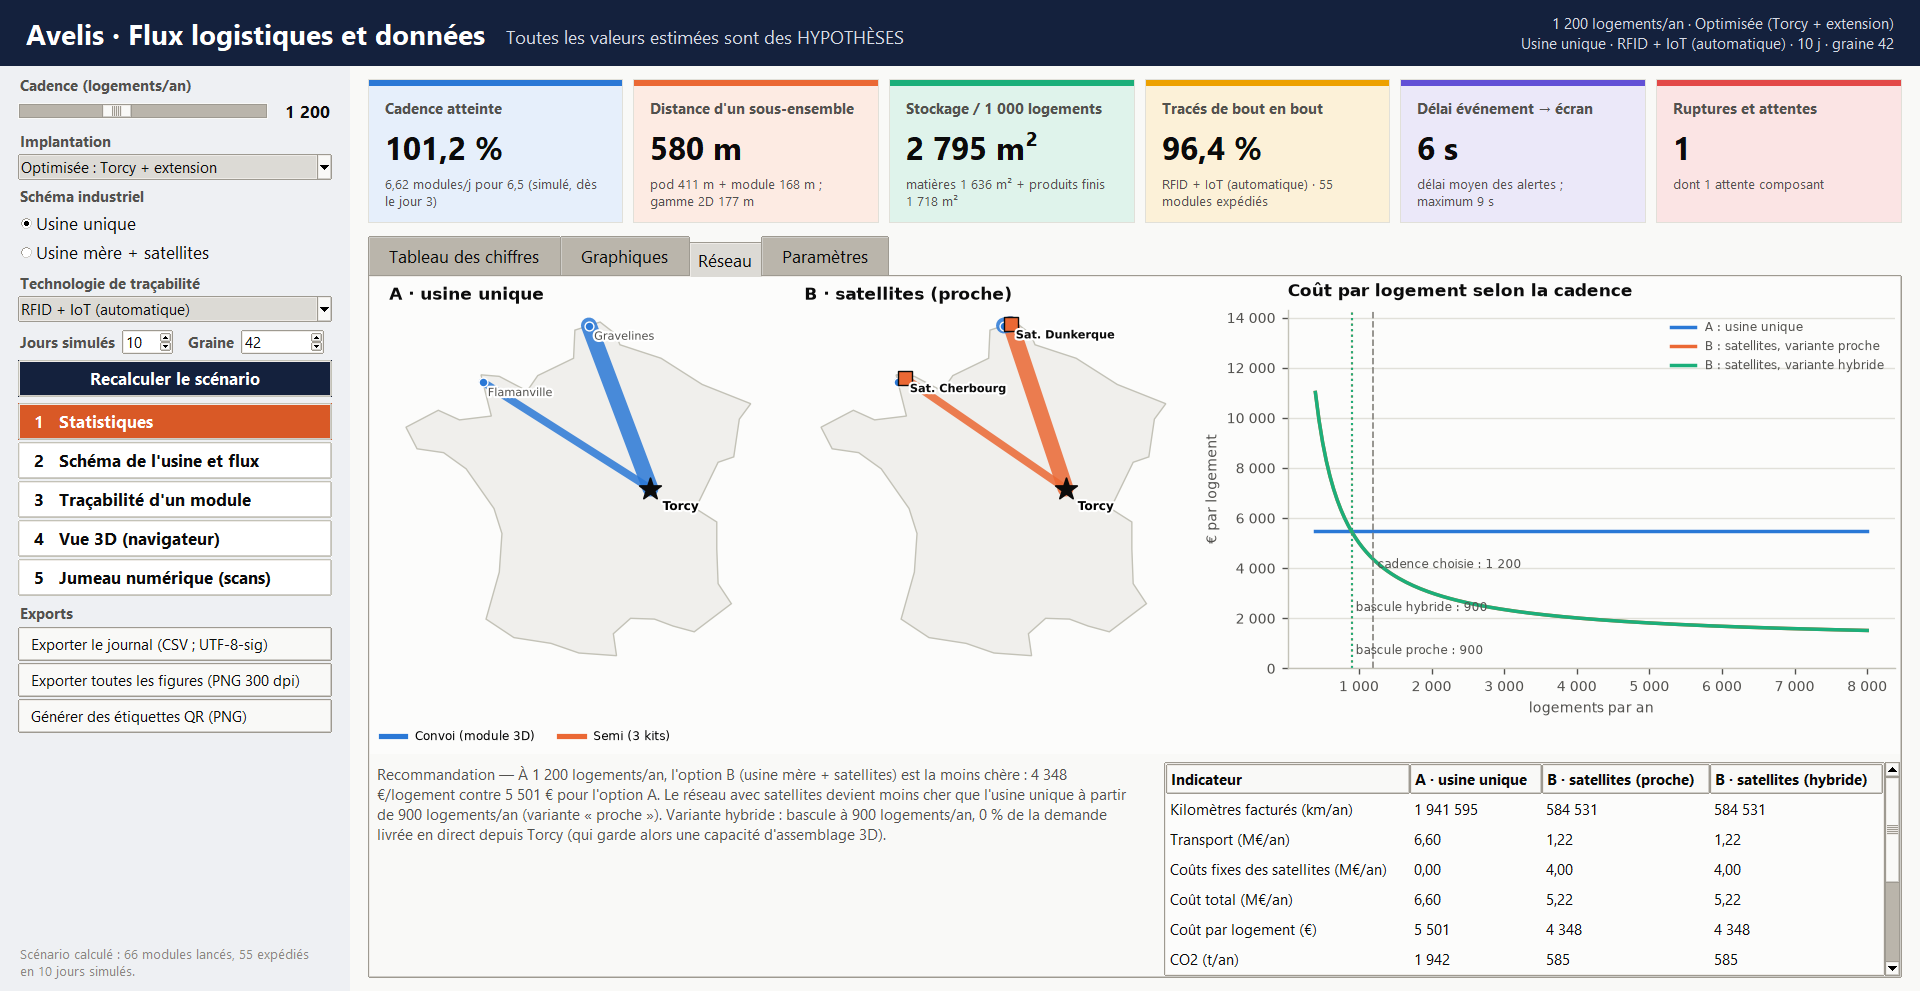
\includegraphics[width=\linewidth]{vue1_reseau_nucleaire.png}
\caption{Onglet \enquote{Réseau} paramétré pour le cas~1 (Gravelines, Flamanville, unités
foraines à Dunkerque et Cherbourg, 1\,200 logements/an) : cartes, coût par logement selon la
cadence et recommandation calculée.}
\end{figure}

\begin{figure}[!htbp]
\centering
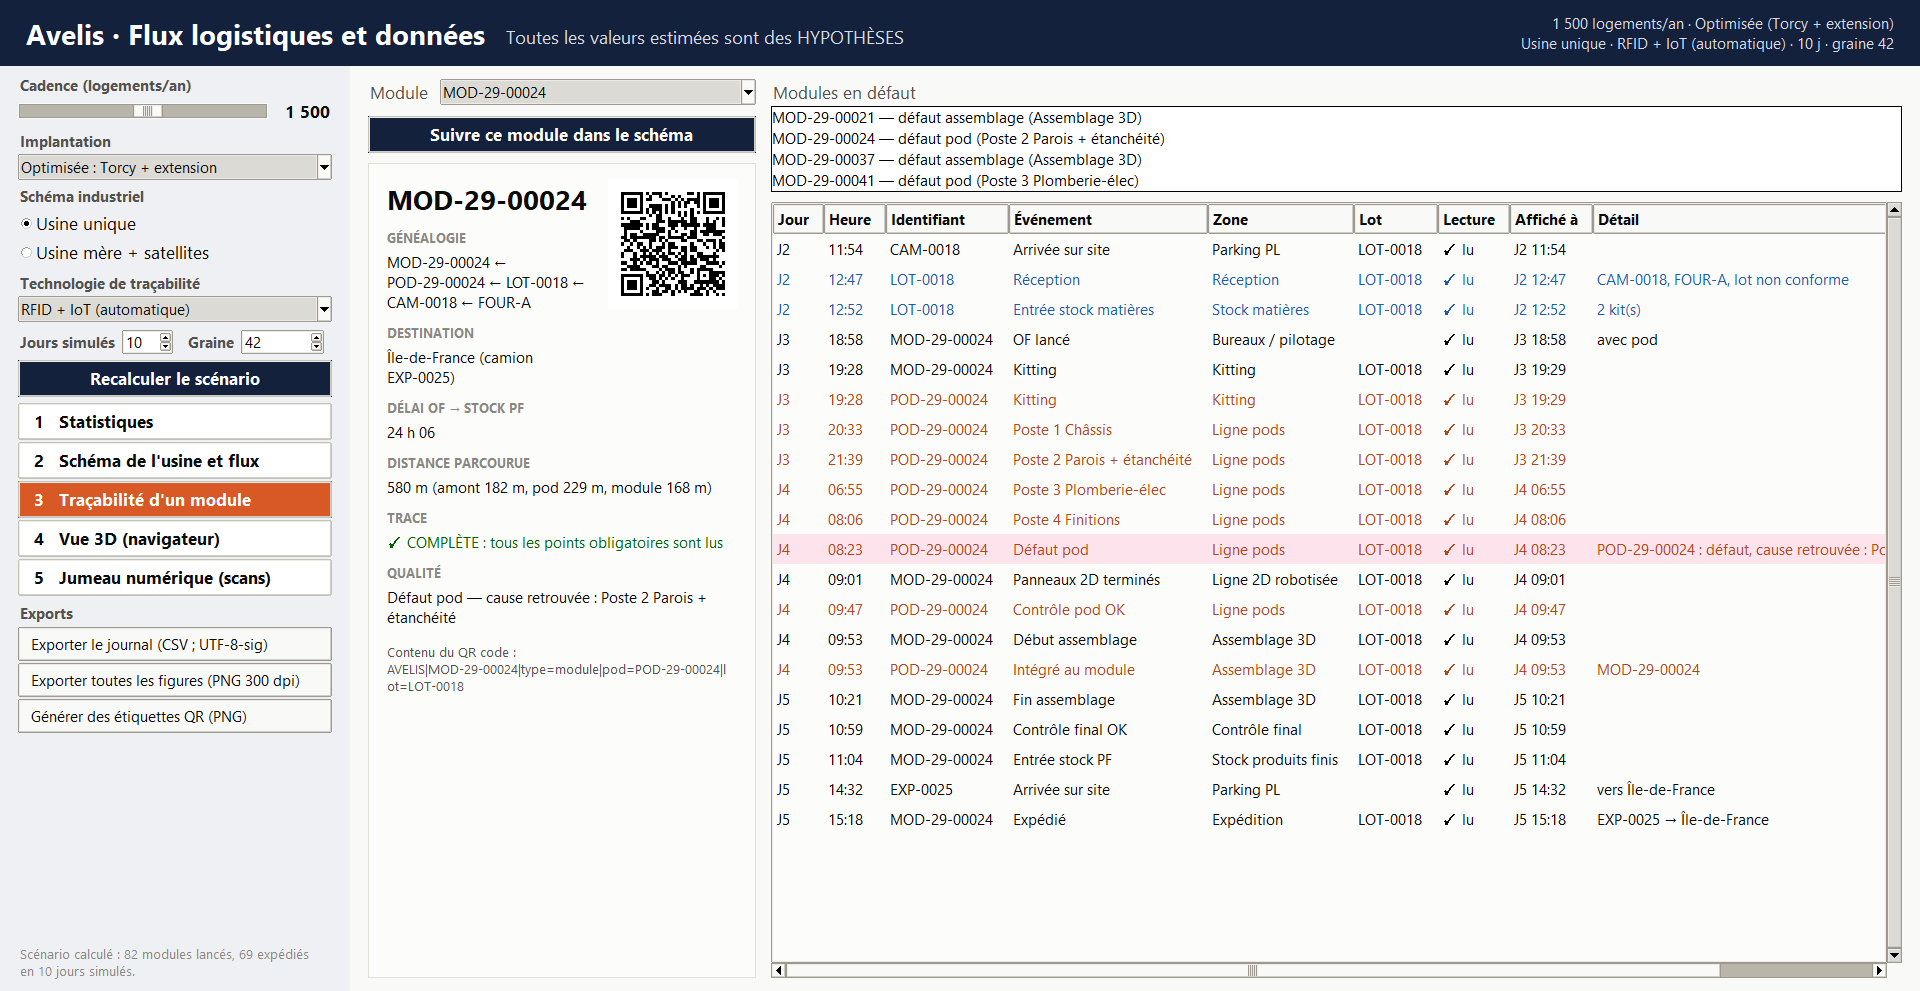
\includegraphics[width=\linewidth]{vue3_tracabilite.png}
\caption{Vue \enquote{Traçabilité d'un module} : généalogie module $\leftarrow$ pod $\leftarrow$
lot $\leftarrow$ camion $\leftarrow$ fournisseur, trace complète et cause du défaut retrouvée,
QR code et chronologie de tous les événements liés.}
\end{figure}

\begin{figure}[!htbp]
\centering
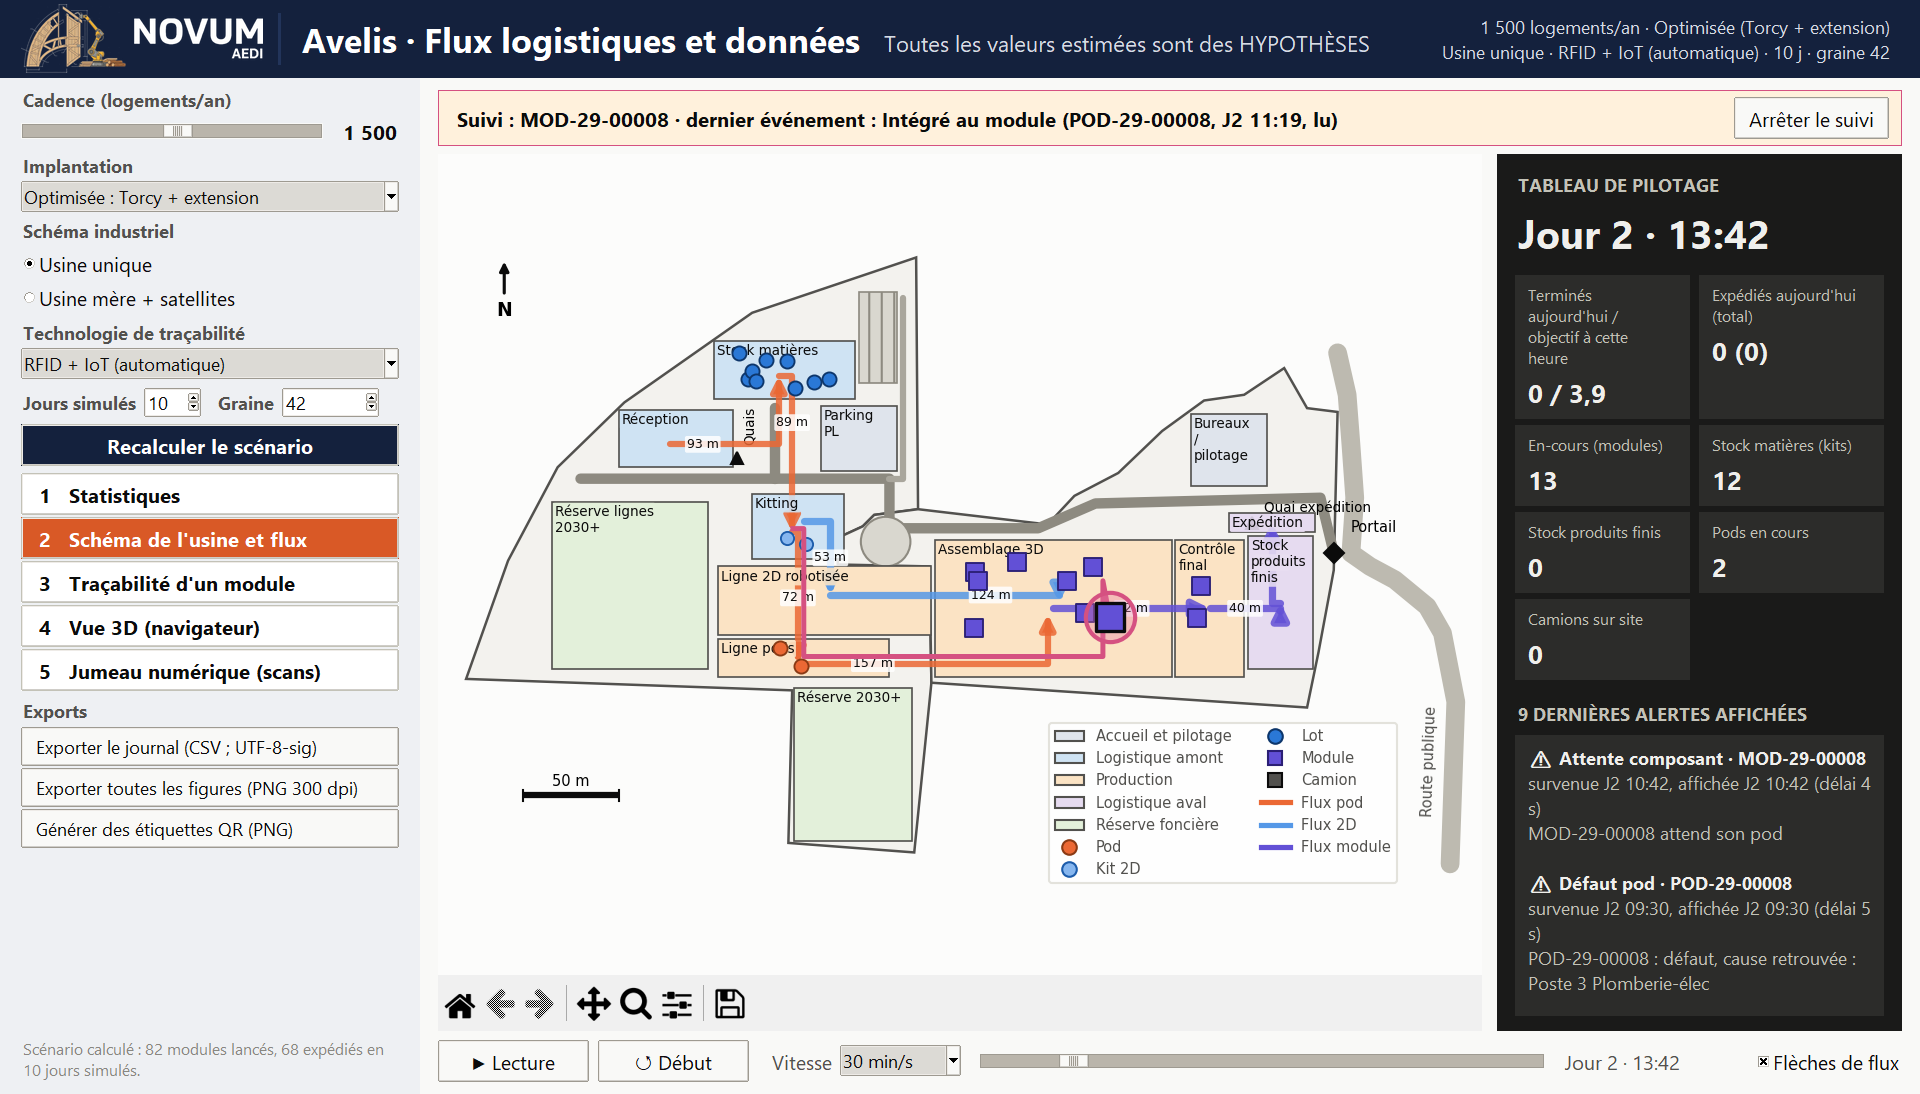
\includegraphics[width=\linewidth]{vue2_suivi.png}
\caption{Mode suivi : le module sélectionné (halo) et le trajet déjà parcouru par son pod.}
\end{figure}

\section{Usage de l'intelligence artificielle générative}\label{ann:ia}

Conformément au règlement du défi, nous déclarons l'usage de l'IA générative. Un journal détaillé
(prompts, vérifications, erreurs détectées) a été tenu pendant tout le projet.

\paragraph{Outil.} Claude Code (application de bureau Claude), modèle Claude Opus~5.5,
éditeur Anthropic. Il a servi à programmer les deux logiciels et à générer les figures et les
captures de ce rapport. Il a aussi assisté la rédaction, qui a été relue et validée par l'équipe.

\paragraph{Prompts.} Ils étaient formulés en français par l'équipe, sur le modèle \enquote{phase
par phase}. En voici des exemples :
\begin{itemize}
  \item \enquote{réalise la phase 2 et la phase 3} ;
  \item \enquote{construis ce jumeau numérique en usine unique avec extension} ;
  \item \enquote{fais en sorte que le jumeau prenne des décisions, mais en mode proposer (il faut
        un humain dans la boucle)} ;
  \item \enquote{modifie l'agencement pour qu'il soit optimisé}.
\end{itemize}
Un cahier des charges figé et un fichier de règles (langue, hypothèses marquées, interdiction
d'ajuster une hypothèse pour atteindre une cible) encadraient chaque demande.

\paragraph{Boucles de rétroaction et vérification.}
\begin{itemize}
  \item Tests écrits avant le code pour le modèle et la simulation. Le dépôt compte 28, 20, 12,
        9, 6, 7 et 17~tests intégrés selon le module.
  \item Valeurs attendues recalculées indépendamment.
  \item Tests d'interface sur 54~combinaisons de paramètres, avec contrôle automatique de la mise
        en page à trois tailles d'écran.
  \item Relecture des captures et confrontation à la théorie : équation~\eqref{eq:trace} et loi
        de Little.
  \item Pour ce rapport, régénération de toutes les données par un script unique
        (\code{rapport/generer\_figures.py}).
\end{itemize}

\paragraph{Hallucinations et erreurs détectées, puis corrigées.}
\begin{itemize}
  \item Une zone de stock débordait du foncier ; elle a été détectée par un test géométrique.
  \item Une première estimation \enquote{à l'œil} du contour du site donnait un rapport
        extension/site de 0,98 au lieu de 0,64 ; elle a été remplacée par une extraction par
        couleur sur le plan.
  \item L'IA supposait un écran à 100\,\% au lieu de 150\,\% ; l'erreur a été corrigée par une
        mesure.
  \item Des pods étaient placés dans les usines satellites, contrairement à la présentation
        d'Avelis ; c'est corrigé.
  \item Les graphiques restaient figés sur le premier scénario, à cause d'un itérateur épuisé.
  \item Une documentation annonçait un anti-double scan de 15~s au lieu de 60~s.
  \item Pendant la rédaction de ce rapport, une figure portait une charge maximale de 85\,\%
        au lieu des 90\,\% du modèle ; l'erreur a été détectée par relecture du code.
\end{itemize}
Les références académiques ont été proposées par l'IA à partir de ses connaissances : l'équipe
en vérifie chaque élément (auteurs, année, DOI) avant la remise. Les faits relatifs aux chantiers
nucléaires proviennent de sources publiques consultées le 4~novembre~2026.

\end{document}
